\documentclass[a4paper,11pt]{article}
% !TeX program = pdflatex
\pdfoutput=1
\pdfminorversion=7
\usepackage[utf8]{inputenc}
\usepackage{CJKutf8}
\AtBeginDocument{\begin{CJK*}{UTF8}{gbsn}}
\AtEndDocument{\clearpage\end{CJK*}}
\usepackage{jheppub}

\usepackage{amsmath,amssymb,latexsym}
\usepackage{braket}
\usepackage{bm}
\usepackage{booktabs}
\usepackage{tabularx}
\usepackage{longtable}
\usepackage{cancel}
\usepackage[svgnames]{xcolor}
\usepackage{hepunits}
\usepackage{mathtools}
\usepackage{graphicx}
\usepackage[most]{tcolorbox}
\usepackage{caption}
\usepackage{tikz}
\usetikzlibrary{calc}
\def\ie{\begin{equation}\begin{aligned}}
\def\fe{\end{aligned}\end{equation}}
\newtcolorbox{proofbox}{
  enhanced, breakable, colback=gray!8, colframe=black,
  boxrule=0.8pt, arc=0pt, outer arc=0pt,
  left=8pt, right=8pt, top=8pt, bottom=8pt,
  before skip=10pt, after skip=10pt
}
\hypersetup{colorlinks=true,linkcolor=blue,citecolor=blue,urlcolor=blue}
\setlength{\emergencystretch}{3em}
\makeatletter
\def\verbatim@font{\normalfont\ttfamily\small}
\makeatother

\title{dS IBP Package 022.0 用户手册}
\author[a]{Su Yingze}
\affiliation[a]{Institute not specified}
\emailAdd{yingze.su@outlook.com}
\abstract{本手册说明 dS IBP package 的费曼规则、massive/massless 指标约定、time 与 loop-momentum IBP、独立变量微分方程 seed、EOM/缩并 canonical、拓扑输入、公开 API、Kira 接口和 tree vertex family。当前发布为 022.0：公开 topology 只使用严格的 vertices/lines Association，顶点以 vertexType 和 externalLegEnergy 定义外腿指数；full 模式使用 J[aList,linePacks,ispList]，time-only 模式使用 J[sectorKey,timeShifts,stateBits]。用户显式分别声明任意命名的 loopExternalMomenta 与 independentExternalMomenta，程序验证结构圈数、routing、声明完备性和动力学坐标，不自动猜角色。package 只生成、序列化和验证关系，不运行 reduction。}

\begin{document}
\sloppy
\setcounter{tocdepth}{1}
\maketitle
\newpage

\section{快速开始与当前边界}

本 package 生成 dS 圈图的 canonical IBP seed，并把关系转换为后端中立的 \texttt{linearData}。当前稳定发布为 022.0，支持 topology-driven 的任意圈数、任意拓扑以及 massive/massless 混合内线；标准入口和正式单文件入口分别为
\begin{verbatim}
package-dSibp/versions/022_dSIBP/
package-dSibp/independent-benchmark/package/package_022.0.wl
\end{verbatim}
工作树只保留当前 022 源码；全部更早源码版本从 Git 历史追溯。022 使用严格的干净输入 schema，并保留标准 context、初始化 metadata、完整 time/loop-momentum 生成元、massive EOM、共同-theta odd-subset contact、contact 可达 sector、跨 sector coincident canonical、Kira serializer/importer 以及 DE/scaling 检查。full 模式保留双端点三槽 line pack；time-only 使用显式 sector key、compact 时间幂和 building-block 状态位列表。

仓库内标准加载与独立 benchmark 单文件加载是两个等价入口，应在新 kernel 中任选其一：
\begin{verbatim}
packageDir = FileNameJoin[{Directory[],"package-dSibp","versions","022_dSIBP"}];
If[!MemberQ[$Path,packageDir],AppendTo[$Path,packageDir]];
Needs["dSIBP`"];

(* 独立 benchmark 的自包含单文件入口： *)
Get["package-dSibp/independent-benchmark/package/package_022.0.wl",
  CharacterEncoding->"UTF-8"];
\end{verbatim}
两者都提供 \texttt{dSIBP`} 公开 context；独立交付文件不依赖主线模块路径。不要在同一 kernel 重复加载两个入口。

全部模块成功加载后，每个 Wolfram kernel 只显示一次简洁引用提醒；Notebook 中的 arXiv 号是
可点击链接，headless kernel 同时保留完整 URL。使用 dSIBP 开展研究时，建议引用：
\begin{enumerate}
  \item Jiaqi Chen and Bo Feng, ``Towards Systematic Evaluation of de Sitter Correlators via Generalized Integration-By-Parts Relations'', \href{https://arxiv.org/abs/2401.00129}{arXiv:2401.00129}.
  \item Jiaqi Chen, Bo Feng and Yi-Xiao Tao, ``Multivariate hypergeometric solutions of cosmological (dS) correlators by d log-form differential equations'', \href{https://arxiv.org/abs/2411.03088}{arXiv:2411.03088}.
  \item Jiaqi Chen, Bo Feng, Zhehan Qin and Yi-Xiao Tao, ``Loop integrals in de Sitter spacetime: The parity-split IBP system and d log-form differential equations'', \href{https://arxiv.org/abs/2604.14549}{arXiv:2604.14549}.
  \item dSIBP package paper, arXiv identifier pending.
\end{enumerate}
程序包论文尚未提供 arXiv 号，因此本手册不为它生成链接或书目信息。

推荐工作流为
\begin{enumerate}
  \item 输入顶点、内线、圈/外动量基、ISP、零点和必要的数值规则；
  \item 用 \texttt{DSInit} 验证输入、ISP 坐标、函数系统与 contact-reachable sectors；
  \item 用 \texttt{DSSeeds} 生成普通 canonical seed batch，并从稳定字段 \texttt{"allSeeds"} 或 \texttt{DSAllSeeds} 取得全部 sector/generator 的一维 general 模板；massive 完整遍历端点四态，masslessFull 只生成 $n_2=0$ 的 $00/10$ quotient representatives；
  \item 模板层立即执行 EOM/symmetry/canonical；再用唯一入口 \texttt{DSGenerateIBP} 显式展开连续指标；
  \item 用 \texttt{DSLinear} 把撒点后的 canonical batch 构造成后端中立 \texttt{linearData}；必要的小规模数值规则只在这一层代入；
  \item 按需调用 \texttt{DSKiraExport}；用户在 package 外运行 reduction；
  \item 有完整外部结果时用 \texttt{DSKiraImport -> DSDE -> DSScaleCheck} 取回并验证。
\end{enumerate}

\begin{proofbox}
解析 seed 只允许小规模生成。禁止默认展开整族解析 IBP，也禁止为了验证做宽范围撒点。所有 WolframScript 检查必须显示消息运行，不能用 \texttt{Quiet} 掩盖问题。
\end{proofbox}

给定下文的 \texttt{case} 后，最短的可执行调用链是
\begin{verbatim}
context = DSInit[case];
templateData = DSSeeds[context,GenerateShrinkSectors->True];
allSeeds = DSAllSeeds[templateData];
seeds = DSGenerateIBP[allSeeds,{0,0}];
linearData = DSLinear[seeds,context];
{context["status"],templateData["dSIBPStatus"],
 seeds["dSIBPStatus"],
 linearData["dSIBPStatus"]}
\end{verbatim}
每个批量接口都返回 Association；必须先检查 \texttt{"status"}，再读取方程或传给下一阶段。

独立 benchmark 的 \texttt{package/examples/} 提供六个应用例子：
\begin{verbatim}
01_mixed_bubble_workflow.wl
02_function_system_hankel.wl
03_single_massive_sunrise/main.wl
04_pure_massive_bubble_closed_loop/main.wl
05_tree_two_vertex_time_ibp/main.wl
06_mix_bubble_tree/main.wl
\end{verbatim}
建议先运行 \path{06_mix_bubble_tree/main.wl}；它展示 018 的显式动量角色、\texttt{ssij/sEe} 初始化、参数重定义、总导数和 cycle/fixed line 数据。\path{03_single_massive_sunrise/main.wl} 使用共同外腿能量 \texttt{kE}、圈外动量 \texttt{kL}、两个在 massless-line 交换下互换的 ISP，以及顶点/平行线 \texttt{symmetryRules}；它只生成全部 contact-reachable sector 的 general IBP seeds 和 \texttt{\{ss11,kE\}} general 参数微分算符。连续指标保持符号，不进入连续撒点、\texttt{linearData}、Kira、DE 或 scaling。

\path{04_pure_massive_bubble_closed_loop/main.wl} 展示外部 Kira 回读、DE 与 scaling；其余例子展示 mixed bubble、一般 \texttt{P,Q,T,W} 函数系统和两顶点 tree pure-time/dlog。examples 不含独立 expected；Kira example 只写输入并取回已有结果，不启动 reduction。

\section{完整例子：mix bubble+tree}

\subsection{先按独立相位能量走通基准流程}

考虑三个时间顶点。\texttt{v1,v2} 之间的 bubble 有两条 cycle lines，动量分别为
\texttt{l1} 与 \texttt{l1+k1+k2}；\texttt{v2,v3} 之间有一条无圈 bridge line，动量为
\texttt{k1+k2}。\texttt{v1} 的另一侧外腿也携带 \texttt{k1+k2}，\texttt{v3} 有两条外腿
\texttt{k1,k2}。输入中的加减法始终是矢量线性组合：
\begin{equation}
 |k_1+k_2|=\sqrt{\operatorname{sp}(k_1+k_2,k_1+k_2)}
 \neq |k_1|+|k_2|
\end{equation}
（一般运动学下）。line 1 是唯一 massive h cycle line，\texttt{nu1} 是它的 Hankel 指标；
line 2 是 massless exponential cycle line，line 3 是 massless exponential bridge。
\texttt{E1,E2,E3} 是三个顶点指数相位的独立标量。package 不从传播子动量或 \texttt{nu1} 推断相位变量。

完整核心输入为
\begin{verbatim}
case = <|
  "name" -> "022BubbleTreeK1K2",
  "vertices" -> {
    <|"id"->v1,"vertexType"->"+","externalLegEnergy"->E1|>,
    <|"id"->v2,"vertexType"->"+","externalLegEnergy"->E2|>,
    <|"id"->v3,"vertexType"->"+","externalLegEnergy"->E3|>
  },
  "lines" -> {
    <|"id"->1,"endpoints"->{v1,v2},"momentum"->l1,
      "nu"->nu1,"massType"->"massive"|>,
    <|"id"->2,"endpoints"->{v1,v2},"momentum"->l1+k1+k2,
      "massType"->"massless"|>,
    <|"id"->3,"endpoints"->{v2,v3},"momentum"->k1+k2,
      "massType"->"massless"|>
  },
  "extLegs" -> {
    {bubbleLeg,v1,k1+k2},{treeLeg1,v3,k1},{treeLeg2,v3,k2}
  },
  "loopMomenta" -> {l1},
  "loopExternalMomenta" -> {k1+k2},
  "independentExternalMomenta" -> {k1,k2},
  "ibpMode" -> "full",
  "ispData" -> {},
  "zeroPointRules" -> {
    a0[v1]->alpha1,a0[v2]->alpha2,a0[v3]->alpha3,
    b0[1]->beta1,b0[2]->beta2,b0[3]->beta3
  },
  "symmetryRules" -> {}
|>;
\end{verbatim}

先查看提案，再初始化：
\begin{verbatim}
proposal = DSKinematics[case];
proposal["selectionTemplate"]

context = DSInit[
  case,
  GenerateDerivativeMetadata -> True,
  ProgressReporting -> True
];
topology = context["topology"];
notation = DSParameterNotation[context];
\end{verbatim}
该输入的必要 loop 方向只有 \texttt{k1+k2}。它的完整一维 Gram 已覆盖 bridge 的模长；
\texttt{k1,k2} 只补齐实际出现的两个独立无圈模长。缺省规则严格为
\begin{verbatim}
sp[k1+k2,k1+k2] -> ss11^2
sp[k1,k1]       -> sE1^2
sp[k2,k2]       -> sE2^2
\end{verbatim}
因此 \texttt{ss11} 是 $|k_1+k_2|$，而 \texttt{sE1+sE2} 才是 $|k_1|+|k_2|$。
短名必须与 \texttt{DSParameterNotation} 返回的原始 \texttt{sp} binding 一起阅读；
\texttt{ssij} 在 $i\ne j$ 时是 Gram 点积坐标的根，不表示 $|k_i+k_j|$。

初始化后可以检查公开原子关系和批量工作流：
\begin{verbatim}
integral = J[
  {0,0,0},
  {{0,0,0},{0,0,0},{"F",0,0}},
  {}
];

timeSeed = dtau[v3,integral,topology];
loopLoopSeed = dqq[1,1,integral,topology];
loopExternalSeed = dqk[1,1,integral,topology];
totalDerivative = ds[ss11^2 integral+sE1 integral,sE1,topology];

seeds = DSSeeds[context];
linearData = DSLinear[seeds,context];
\end{verbatim}
massive/massless cycle full pack 都是 \texttt{\{b,n1,n2\}}；fixed bridge full pack 是
\texttt{\{"F",n1,n2\}}，其中 \texttt{"F"} 是数据 sentinel，不是幂指标。bridge 的动量幂进入
sector 的结构化 prefactor，不伪造 \texttt{b} 指标。解析 seed 不要求给数值规则。即使为了缩小 Kira 系数域固定 \texttt{dim}、
\texttt{nu1}、zero-point 或 normalization，所有准备生成 DE 的变量
\texttt{\{ss11,sE1,sE2,E1,E2,E3\}} 仍必须保持符号；不得在 export 前给它们数值。

\subsection{方案一：保留两条外腿，把模长和选作坐标}

如果同一顶点的两个外腿指数需要合并成
\begin{equation}
 E_0=|k_1|+|k_2|,
\end{equation}
是否采用 $E_0$ 是用户的运动学参数选择，不由 package 猜测。保留原 topology 时，先把
\texttt{v3} 的相位能量显式改为 \texttt{E0}，再做满秩坐标重定义：
\begin{verbatim}
boundCase = Join[
  case,
  <|"vertices"->ReplacePart[
      case["vertices"],{3,"externalLegEnergy"}->E0
    ]|>
];
boundContext0 = DSInit[boundCase,GenerateDerivativeMetadata->True];

boundContext = DSRedefineParameters[boundContext0,{
  sp[k1+k2,k1+k2] -> ss11^2,
  sp[k1,k1]       -> (E0-sE2)^2,
  sp[k2,k2]       -> sE2^2
}];
\end{verbatim}
数学上这正是 \texttt{sE1->E0-sE2,sE2->sE2}，但公开 API 的规则左端必须写
\texttt{baseCoordinateOrder} 中的原始 \texttt{sp[...]}，不能直接写 \texttt{sE1->...}。
该坐标图的可求导变量为
\begin{verbatim}
{ss11,E0,sE2,E1,E2}
\end{verbatim}
其中 \texttt{E0} 只出现一次；\texttt{ds[expr,E0,boundContext]} 同时对显式系数、模长 binding
和 \texttt{v3} 相位求导。平方规则选择了 $|k_1|=E_0-sE_2$ 的物理支，使用者应在所研究区域保证
$E_0>s_E2>0$；若需要别的分支，必须显式更换参数化。

只改坐标而仍令 \texttt{v3->E3}，不会建立 $E_3=E_0$；相反，只令 \texttt{v3->E0} 而不重定义
两个模长，也不会告诉 package $E_0=sE1+sE2$。这两部分必须同时给出。

\subsection{方案二：从输入起采用单一有效外腿}

另一种做法是把 \texttt{v3} 的两条外腿替换成一条有效外腿。此时 topology metadata 已改变，
不能把它当作上一个 family 的纯坐标改名。为避免同一符号既作矢量又作标量，使用 \texttt{p0}
标记有效外腿三动量，用 \texttt{E0} 标记其模长和顶点相位：
\begin{verbatim}
singleLegCase = Join[case,<|
  "name" -> "018BubbleTreeSingleEffectiveLeg",
  "extLegs" -> {
    {bubbleLeg,v1,k1+k2},
    {treeLeg0,v3,p0}
  },
  "independentExternalMomenta" -> {p0},
  "vertices" -> ReplacePart[
    case["vertices"],{3,"externalLegEnergy"}->E0
  ]
|>];

singleLegContext0 = DSInit[
  singleLegCase,
  GenerateDerivativeMetadata->True
];
singleLegContext = DSRedefineParameters[singleLegContext0,{
  sp[k1+k2,k1+k2] -> ss11^2,
  sp[p0,p0]       -> E0^2
}];
\end{verbatim}
此时 \texttt{v3} 只有一条外腿，独立变量为 \texttt{\{ss11,E0,E1,E2\}}。package 只知道
$|p_0|=E_0$；“这个 $E_0$ 对应原问题的 $|k_1|+|k_2|$”是用户在两个不同 topology 之间建立的
外部物理对应，不再能从新输入中恢复原来的两个独立模长，也不能分别对它们求导。若后续仍需要
$k_1,k_2$ 的独立变化、交换对称性或软极限，应使用方案一而不是删除两条外腿。

\section{SK 费曼规则到积分族}

\subsection{顶点规则}

每个时间顶点 $v$ 有共形时间 $\tau_v<0$ 和 SK 分支 $\sigma_v=\pm$。本 package 使用
\begin{equation}
  \sigma_v=+:\quad e^{-iE_v\tau_v},
  \qquad
  \sigma_v=-:\quad e^{+iE_v\tau_v}.
\end{equation}
因此外腿相位对 time-IBP 的贡献为
\begin{equation}
  \partial_{\tau_v}e^{-iE_v\tau_v}=-iE_v e^{-iE_v\tau_v},
  \qquad
  \partial_{\tau_v}e^{+iE_v\tau_v}=+iE_v e^{+iE_v\tau_v}.
  \label{vertexPhaseRule}
\end{equation}
$E_v$ 表示连接该顶点的所有外腿模长在指数中形成的打包能量。它不一定是进入圈内线动量的外部向量。

\subsection{内线的四种类型}

设内线 $e$ 的有序端点为 $\{u_e,v_e\}$，动量为
\begin{equation}
 \bm Q_e=\sum_{\ell=1}^{L}c_{e\ell}\bm q_\ell
        +\sum_{j=1}^{K}d_{ej}\bm k_j,
 \qquad q_e=|\bm Q_e|.
\end{equation}
端点的 SK 符号决定传播子类型：
\begin{center}
\begin{tabular}{lll}
\toprule
质量类型 & 端点分支 & 指标包\\
\midrule
massive & 同分支 $++/--$ & \texttt{\{b[e],n[e,1],n[e,2]\}}\\
massive & 异分支 $+-/-+$ & \texttt{\{b[e],n[e,1],n[e,2]\}}\\
massless & 同分支 $++/--$ & \texttt{\{b[e],n[e,1],n[e,2]\}}\\
massless & 异分支 $+-/-+$ & \texttt{\{b[e],0,0\}}\\
\bottomrule
\end{tabular}
\end{center}
同分支线含 theta ordering，称为 full line；异分支线没有 theta 导数产生的 shrink，称为 cross line。massive cross 仍有两个 Hankel 端点态；massless cross 是单个指数乘积，因此两个离散槽固定为零。表中给出 cycle schema；fixed line 把第一槽 \texttt{b[e]} 换成 sentinel \texttt{"F"}。

\subsection{Bubble 图作为输入例子}

下图只是一个 topology 输入例子，不代表生成器硬编码 bubble。两条内线可分别选为 massive/massless full/cross；只需改变 family metadata，统一积分 Head 不变。

\begin{center}
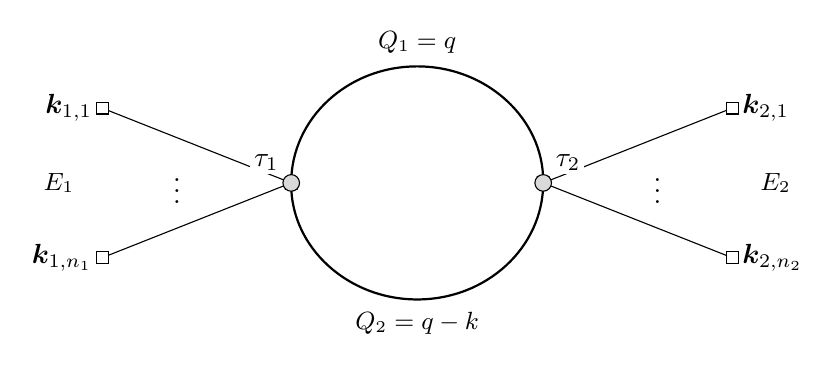
\begin{tikzpicture}[scale=1.0, every node/.style={inner sep=1.5pt}]
  \coordinate (vL) at (0,0);
  \coordinate (vR) at (3.2,0);
  \coordinate (lU) at (-2.4,0.95);
  \coordinate (lD) at (-2.4,-0.95);
  \coordinate (rU) at (5.6,0.95);
  \coordinate (rD) at (5.6,-0.95);
  \draw (vL) -- (lU) node[left=2pt] {$\bm{k}_{1,1}$};
  \draw (vL) -- (lD) node[left=2pt] {$\bm{k}_{1,n_1}$};
  \draw (vR) -- (rU) node[right=2pt] {$\bm{k}_{2,1}$};
  \draw (vR) -- (rD) node[right=2pt] {$\bm{k}_{2,n_2}$};
  \node[fill=white,inner sep=1pt] at (-1.45,0) {$\vdots$};
  \node[fill=white,inner sep=1pt] at (4.65,0) {$\vdots$};
  \draw[->,thick] (vL) arc[start angle=180,end angle=0,x radius=1.6,y radius=1.48];
  \draw[->,thick] (vR) arc[start angle=0,end angle=-180,x radius=1.6,y radius=1.48];
  \node[fill=white] at (1.6,1.78) {\small $Q_1=q$};
  \node[fill=white] at (1.6,-1.78) {\small $Q_2=q-k$};
  \node[fill=white] at (-2.95,0) {\small $E_1$};
  \node[fill=white] at (6.15,0) {\small $E_2$};
  \filldraw[fill=gray!30,draw=black] (vL) circle (3pt);
  \filldraw[fill=gray!30,draw=black] (vR) circle (3pt);
  \node[fill=white,anchor=south east] at (-0.10,0.10) {$\tau_1$};
  \node[fill=white,anchor=south west] at (3.30,0.10) {$\tau_2$};
  \filldraw[fill=white,draw=black] ($(lU)+(-0.075,0.075)$) rectangle ++(0.15,-0.15);
  \filldraw[fill=white,draw=black] ($(lD)+(-0.075,0.075)$) rectangle ++(0.15,-0.15);
  \filldraw[fill=white,draw=black] ($(rU)+(-0.075,0.075)$) rectangle ++(0.15,-0.15);
  \filldraw[fill=white,draw=black] ($(rD)+(-0.075,0.075)$) rectangle ++(0.15,-0.15);
\end{tikzpicture}
\end{center}

例如 mixed bubble 可取 $Q_1=q$ 为 massive，$Q_2=q-k$ 为 massless。pure massless bubble 则把两线都设为 massless。顶点符号从 $++$ 改成 $+-$ 时，两条线自动从 full 变为 cross；不是换一套积分 Head。

\section{按 mode 固定的三参数积分表示}

所有 top/sub-sector 都使用三个正式槽位
\begin{equation}
 \boxed{
 J\!\left[
   \{a_v\},
   \{\mathrm{pack}_e\},
   \{n_{\mathrm{isp},r}\}
 \right]}
 \equiv
 \texttt{J[aList,linePacks,ispList]}.
 \label{threeSlotJ}
\end{equation}
三个槽位分别是
\begin{enumerate}
  \item \texttt{aList}：当前 sector 的独立时间变量幂次；
  \item \texttt{linePacks}：按固定 line slot 排列的传播子/缩并线指标包；
  \item \texttt{ispList}：ISP 的正式指标槽，不是附注 metadata。
\end{enumerate}

式~\eqref{threeSlotJ} 是 full 模式的 schema。020 的 time-only 公开 schema 为
\begin{equation}
 \boxed{J[\texttt{sectorKey},\texttt{timeShifts},\texttt{stateBits}]}.
 \label{timeOnlyPublicJ}
\end{equation}
\texttt{sectorKey} 是 root propagator 顺序的定长字符串；\texttt{timeShifts} 按当前 sector 的 compact vertex components 排列；\texttt{stateBits} 是 $n_i$ 类离散函数态，不是第二套 sector key。初始化一旦选择 mode，公开入口就只接受对应 schema。

实际幂次包含初始化零点：
\begin{equation}
 A_v=a_v+a0_v,\qquad
 B_e=b_e+b0_e,\qquad
 B^S_e=bS_e+bS0_e.
\end{equation}
质量、$\nu_e$、端点、SK 符号、动量表达式、顶点能量、外不变量名称和 symmetry rules 都不写入 $J$。

theta 导数缩并线时，pack 变为
\begin{equation}
  \mathrm{pack}_e=\{bS_e\}.
\end{equation}
delta 函数合并两个时间变量，所以 \texttt{aList} 只保留一个代表顶点槽；原顶点到 compact slot 的映射保存在 \texttt{sectorMetadataList}。line slot 始终保留，不能删除 $bS_e$。

\section{Massive 导数、EOM 与缩并}

\subsection{端点导数与即时 EOM}

massive full/cross 的两个端点态均取 $n_{e,r}=0,1$。time 导数先产生
\begin{equation}
 \partial_{\tau_r}:\qquad
 -J[\ldots,\{b_e-1,n_{e,r}+1,\ldots\},\ldots].
\end{equation}
若 $n_{e,r}=1$，二阶态必须立刻 EOM。对 h：
\begin{equation}
 J[n_{e,r}=2]
 =-J[n_{e,r}=0]
  -(2\nu_e+1)J[a_r-1,b_e+1,n_{e,r}=1].
 \label{massiveEOM}
\end{equation}
对裸 H：
\begin{equation}
 J_H[n_{e,r}=2]
 =-J_H[n_{e,r}=0]
  -J_H[a_r-1,b_e+1,n_{e,r}=1]
  +\nu_e^2J_H[a_r-2,b_e+2,n_{e,r}=0].
 \label{bareHEOM}
\end{equation}
另一端点指标不变。最后一项就是 $\nu_e^2/x^2$ 二次 pole；loop-momentum 导数若产生 $n=2$，同样在 seed 层立即使用对应 EOM。当前 018 由统一函数系统编译这些递推；旧版内置公式只作为历史基线。

\subsection{通用 $2\times2$ 函数系统输入}

当前 018 对每条 massive line 输入
\begin{equation}
 f''+P(x)f'+Q(x)f=0,
 \qquad \mathbf F=T(x)(f,f')^T,
 \qquad x=-\xi\tau,
\end{equation}
其中 $P$ 是一阶导系数、$Q$ 是零阶系数，$T$ 缺省为单位矩阵；还必须给原始导数基底的完整 Wronskian $W$。初始化层统一生成
\begin{equation}
 A_0=\begin{pmatrix}0&1\\-Q&-P\end{pmatrix},
 \qquad
 A_T=T'T^{-1}+TA_0T^{-1},
 \qquad
 W_T=\det(T)W.
\end{equation}
IBP 的 time/radial 导数只调用由 $A_T$ 编译的移位数据，theta shrink 只调用由 $W_T$ 编译的数据；不在 IBP 层重算 $P,Q,T,W$。缺省 massive 模式是 h，直接取 $P_h=(2\nu+1)/x$、$Q_h=1$、$T=I_2$ 与完整 $W_h$，所以 $W_T=W_h$。裸 H 是另一个 $T=I_2$ preset。若从 H 输入经一般基变换构造 h，则
\begin{equation}
 \mathbf h=x^{-\nu}\begin{pmatrix}1&0\\-\nu/x&1\end{pmatrix}\mathbf H,
 \qquad W_h=x^{-2\nu}W_H.
\end{equation}
该编译接口已在当前 018 实现；显式 $W_T$ 只作 $W_T=\det(T)W$ 的一致性校验。缺省 h、裸 H、一般 $T$ 和非法输入由函数系统专项检查覆盖，h/H 另有独立物理 benchmark。Wronskian 的标准推导见技术笔记专门 subsection。

用户输入一般函数系统时，在对应 massive line 中加入
\begin{verbatim}
"functionSystem" -> <|
  "variable" -> x,
  "P" -> Pexpr,
  "Q" -> Qexpr,
  "T" -> {{t11,t12},{t21,t22}},
  "W" -> Wexpr,
  "WT" -> Automatic,
  "shrinkBShift" -> 1,
  "shrinkZeroPointShift" -> zeroShift
|>
\end{verbatim}
也可在放入 line 前调用
\begin{verbatim}
compiled = compileFunctionSystem[functionSystem];
compiled["status"]
compiled["AT"]
compiled["WT"]
\end{verbatim}
检查编译结果。\texttt{T} 省略时为单位矩阵；输入必须通过可逆性、Abel/Wronskian 一致性和有限 Laurent 编译门禁。\texttt{shrinkBShift} 与 \texttt{shrinkZeroPointShift} 是由函数系统和 Wronskian 决定的物理编译数据，不是普通显示或 basis 选项。使用内建 h/H preset 时应保留缺省值；一般函数系统也应优先让编译结果决定这两个量。

\subsection{Massive theta shrink}

只有 massiveFull 且 $n_{e,1}+n_{e,2}=1$ 时有 Wronskian shrink。端点 $r$ 的系数为
\begin{equation}
 {\cal C}_e(-1)^{n_{e,r}+V_{\pm}},
 \qquad
 V_{\pm}=
 \begin{cases}
 1,&++,\\
 0,&--,
 \end{cases}
 \qquad
 {\cal C}_e=\frac{4i}{\pi}e^{\pi\,\mathrm{Im}\nu_e}.
 \label{massiveShrinkSign}
\end{equation}
当前实现允许 line/case 显式覆盖 sign offset，但默认值遵循式~\eqref{massiveShrinkSign}。

对 $h$ 模式：
\begin{align}
 a_{\rm merged}&=a_u+a_v-1,&
 a0_{\rm merged}&=a0_u+a0_v-2\nu_e,\\
 bS_e&=b_e+1,&
 bS0_e&=b0_e+2\nu_e.
\end{align}
对 $H$ 模式整数移位相同，但两个 $2\nu_e$ zero-point shift 都为零。massiveCross 没有 theta shrink。

因此现行缺省值及其实际 child 映射为
\begin{center}
\begin{tabular}{c|c|c|c|c|c}
\toprule
模式 & $(s,z)$ & $a_{\rm merged}$ & $a0_{\rm merged}$ & $bS_e$ & $bS0_e$\\
\midrule
h & $(1,2\nu_e)$ & $a_u+a_v-1$ & $a0_u+a0_v-2\nu_e$ & $b_e+1$ & $b0_e+2\nu_e$\\
H & $(1,0)$ & $a_u+a_v-1$ & $a0_u+a0_v$ & $b_e+1$ & $b0_e$\\
\bottomrule
\end{tabular}
\end{center}
这里 $s$ 进入整数指标，$z$ 进入 zero point。对带圈动量的 line，contact 支持 $n_{e,1}+n_{e,2}=1$，故两种缺省模式都满足
\begin{equation}
 b_e+n_{e,1}+n_{e,2}\equiv b_e+1=bS_e\pmod 2.
\end{equation}
所以缺省 h/H shrink 不改变 subsector parity。h 的 $2\nu_e$ 是 zero point 而非整数 seed 指标，H 的 zero-point shift 为零；fixed/non-loop line 不进入 parity 判定。对 fixed/non-loop line 不保留 $b/bS$ 指标槽，缺省 $z$ 进入 target sector 的结构化 prefactor，normalized contact coefficient 保留整数部分对应的模长幂 $r^{-s}$。

一般不建议用户修改 \texttt{shrinkBShift} 或 \texttt{shrinkZeroPointShift}。若物理函数系统确实要求 override，必须同时重新建立 child-sector zero point、跨 sector normalization coefficient 和 parity metadata；只改一个 shift 而沿用其它缺省数据会得到不一致的 reduction/DE。若相对缺省的 zero-point 重基不能精确判定为整数，相应 sector 的 parity 功能应关闭。需要额外吸收显式模长幂时，应通过后续 master/basis 选择处理，而不是另改 shrink shift。

\section{Massless 双端点 quotient 与 time-IBP}

\subsection{有序端点定义}

对有序端点 \texttt{\{u,v\}}，令 $\Delta=\tau_u-\tau_v$。masslessFull 的同分支符号记为 $\sigma=+1$ 对 $++$、$\sigma=-1$ 对 $--$：
\begin{align}
 M_0&=\theta(\Delta)e^{-i\sigma q\Delta}
      +\theta(-\Delta)e^{+i\sigma q\Delta},\\
 M_1&=-\theta(\Delta)e^{-i\sigma q\Delta}
      +\theta(-\Delta)e^{+i\sigma q\Delta}.
 \label{masslessM01}
\end{align}
第一端点定义 $M_1$ 的方向。交换端点时 $M_0$ 不变、$M_1$ 变号。018 的公开双端点态记为 $F_{n_1n_2}$，并用
\begin{equation}
 F_{00}=M_0,\qquad F_{10}=M_1,\qquad
 F_{01}=-F_{10},\qquad F_{11}=-F_{00}
 \label{masslessDoubleEndpoint}
\end{equation}
定义 quotient。正式 $J$ 始终保存三槽 $\{b_e,n_{e,1},n_{e,2}\}$，两个端点指标均只取 $0,1$；relation 层以 $n_{e,2}\to0$ 为 canonical 方向，不建立 massless $n=2$ 状态。

这里的 $F_{11}=-F_{00}$ 已抽出每次端点导数的 $\pm i\sigma q$。原始时间导数关系仍为 $\{11\}=+q^2\{00\}$：cycle line 由两次 $b\to b-1$ 承载 $q^2$，fixed/独立外动量 line 由导数算符显式乘两次模长参数。用户不需要为同一代数类重复生成 source seeds；\texttt{DSSeeds} 只生成 $00/10$，但导数产生的 $01/11$ 会连同这些系数立即约回。返回的 \texttt{seedTemplateSummary["discreteStateAudits"]} 记录 raw 四态数、代表态数、删除数和 canonical direction。

每条 massless line 仍保留自己的三槽 pack；只有共享同一当前代表顶点对的 time boundary 按共同 theta 组合。fixed line 对应写成 $\{\texttt{"F"},n_{e,1},n_{e,2}\}$。

\subsection{两个端点的 regular 与 delta 规则}

由式~\eqref{masslessM01}，
\begin{align}
 \partial_{\tau_u}M_n
 &=+i\sigma q\,M_{1-n}
   -2n\,\delta(\tau_u-\tau_v),\\
 \partial_{\tau_v}M_n
 &=-i\sigma q\,M_{1-n}
   +2n\,\delta(\tau_u-\tau_v).
 \label{masslessTimeRules}
\end{align}
对一般公开状态先应用式~\eqref{masslessDoubleEndpoint}。在 canonical representative $\{b,n,0\}$ 上，四个基本端点检查为
\begin{center}
\begin{tabular}{ccl}
\toprule
$n$ & 端点 & regular 指标变化与系数\\
\midrule
0 & 第一端点 & $+i\sigma\,\{b-1,1,0\}$\\
0 & 第二端点 & $-i\sigma\,\{b-1,1,0\}$\\
1 & 第一端点 & $+i\sigma\,\{b-1,0,0\}$\\
1 & 第二端点 & $-i\sigma\,\{b-1,0,0\}$\\
\bottomrule
\end{tabular}
\end{center}
同一端点连续作用两次，regular 部分回到原 canonical representative：
\begin{equation}
 \partial_{\tau_u}^2:\quad
 -J[\{b-2,n,0\}],
 \qquad
 \partial_{\tau_v}^2:\quad
 -J[\{b-2,n,0\}].
\end{equation}

\subsection{Massless shrink 与抵消}

公开奇数端点态 $n_1+n_2=1$ 才产生 theta-delta；在 canonical representative 中即 $\{n_1,n_2\}=\{1,0\}$：
\begin{equation}
 \partial_{\tau_u}:\ -2\,\delta(\tau_u-\tau_v),
 \qquad
 \partial_{\tau_v}:\ +2\,\delta(\tau_u-\tau_v).
 \label{masslessDeltaSigns}
\end{equation}
massless shrink 没有 Hankel Wronskian prefactor，也没有 $2\nu$ shift：
\begin{equation}
 a_{\rm merged}=a_u+a_v,\qquad
 a0_{\rm merged}=a0_u+a0_v,\qquad
 bS_e=b_e,\qquad bS0_e=b0_e.
 \label{masslessShrink}
\end{equation}

这里缺省 compiled shift 是 $(s,z)=(0,0)$。“没有 shift”的准确含义是 shrink 不新增任何整数幂或 zero-point 幂吸收。对 cycle line，式~\eqref{masslessShrink} 直接保留 $bS_e=b_e$、$bS0_e=b0_e$。对 fixed/non-loop line，source sector 已有的模长幂必须保存在完整 $N_s$；target 收缩后按其自身 $N_t$ 归一化。contact 一律先生成裸核系数 $c_{\rm raw}$，再写成
\begin{equation}
 c_{\rm raw}\,\frac{N_s}{N_t}\,J_t.
\end{equation}
因此 atomic fixed massless $++$ 的 contact 系数精确为 $-2/sE1^{\beta_1}$，不是 $-2$。同一 \texttt{sectorPrefactorData} 同时服务 contact、\texttt{ds/DSDE} 与反向被积函数恢复，禁止在任一 consumer 另猜一次模长幂。

massless 的 subsector parity 不保持原 offset。018 双端点表示中 contact 支持满足 $n_1+n_2=1$，而 $bS=b$，所以若 parent 使用 $b+n_1+n_2$ 分级，
\begin{equation}
 b+n_1+n_2=b+1=bS+1\pmod 2.
 \label{manualMasslessContactParity}
\end{equation}
因此 cycle massless contact 使 child-sector parity offset 相对 parent 翻转 1；fixed/non-loop massless line 不参与 parity，没有这次翻转。多线 simultaneous contact 按被 shrink 的 massless cycle line 数模 2 累加。018 不自动给 pure massless family 启用 parity；mixed h/H 系统一旦使用已认证 root parity，massless cycle transition 必须携带上述 affine offset，不能套用 h/H 的“缺省不变”。

缩并后，剩余传播子的两个原端点可能映到同一个 active vertex。此时：
\begin{enumerate}
  \item time 导数必须同时作用于两个端点，不能只取第一个匹配；
  \item 两个 regular 端点贡献按式~\eqref{masslessTimeRules} 抵消；
  \item 两个 theta-delta 贡献的 $-2/+2$ 系数相消，不再产生 shrink 项；
  \item 反对称态 $n=1$ 在 coincident endpoint 恒为零。
\end{enumerate}
这个零关系也必须作用于从 top 方程产生的目标 sub-sector 项。当前实现根据每个 $J$ 中已经变成单元素 pack 的 shrunk lines，重建目标 sector 的顶点代表映射，再判定 coincident $n=1$；不能只读取 source top 的 endpoints。

对 $+-$ 或 $-+$ masslessCross，没有 $n$、theta 或 shrink。端点 regular 系数由该端点分支决定：
\begin{equation}
 +\text{端点}:\ +i\,\{b-1\},
 \qquad
 -\text{端点}:\ -i\,\{b-1\}.
\end{equation}

\subsection{同一顶点对多条 full lines}

同一当前代表顶点对的 massive/massless full lines 共享时间差 $\Delta$。写
\begin{equation}
 G_e=\theta(\Delta)A_e+\theta(-\Delta)B_e,
\end{equation}
则整个 bundle 的 boundary 只有
\begin{equation}
 \delta(\Delta)\left(\prod_eA_e-\prod_eB_e\right).
\end{equation}
定义 $J_e=(A_e+B_e)/2$、$D_e=A_e-B_e$，可保持现有逐线 pack：
\begin{equation}
 \prod_eA_e-\prod_eB_e
 =\sum_{\substack{\varnothing\ne S\subseteq B\\|S|\ {\rm odd}}}
 2^{1-|S|}\prod_{e\in S}D_e\prod_{e\notin S}J_e.
 \label{manualOddSubsetContact}
\end{equation}
一次事件可同时 shrink 任意非空奇数条 bundle 线，系数为 $2^{1-|S|}$，但只合并一次顶点且只含一个 delta。两线只有 single contacts；三线另有系数 $1/4$ 的 triple contact。未选择的 coincident full lines 立即应用 massless $n=1$ 为零和 massive endpoint-swap canonical，不会再次产生 theta boundary。

sector 只允许连接两个不同当前代表类的 contact 事件，按 BFS 枚举；事件之间形成 forest，但单个事件可选择多条平行线。单传播子的对称 equal-time 值取 $\theta(0)=1/2$，但不把它作为 $\delta\theta^m$ 的点值乘法规则。保留逐线 theta 时，统一 Gaussian mollifier 给出的线别积分在求和后严格等价于式~\eqref{manualOddSubsetContact}。

例如三条同向 masslessFull 线均取 $n_1=n_2=n_3=1$，并从第一有序端点求导。此时每条线的对称等时因子为零、contact difference 为 $-2$，所以三个 single-contact 项都因未选中线的等时因子为零而消失，只剩
\begin{equation}
 \frac14(-2)^3=-2.
\end{equation}
指标上即
\begin{align}
 &J[\{a_u,a_v\},
   \{\{b_1,1,0\},\{b_2,1,0\},\{b_3,1,0\}\},\{\cdots\}]
 \nonumber\\
 &\qquad\longrightarrow
 -2J[\{a_u+a_v\},\{\{b_1\},\{b_2\},\{b_3\}\},\{\cdots\}].
\end{align}
三个 pack 同时 shrink，但只合并一次顶点且没有额外 massless 幂次 shift。共同-theta与 Gaussian 逐线方案的完整推导、massive $W_T$ 例子和等价条件见技术笔记附录。

\section{Topology、标量积、ISP 与外腿能量}

\subsection{输入骨架}

\begin{verbatim}
case = <|
  "name" -> "mixedBubble",
  "vertices" -> {
    <|"id"->v1,"vertexType"->"+",
      "externalLegEnergy"->Sqrt[sp[kE,kE]]|>,
    <|"id"->v2,"vertexType"->"+","externalLegEnergy"->E2|>
  },
  "lines" -> {
    <|"id"->1,"endpoints"->{v1,v2},"momentum"->q,
      "nu"->nuM,"massType"->"massive"|>,
    <|"id"->2,"endpoints"->{v1,v2},"momentum"->q-k,
      "massType"->"massless"|>
  },
  "loopMomenta" -> {q},
  "loopExternalMomenta" -> {k},
  "independentExternalMomenta" -> {kE},
  "ibpMode" -> "full",
  "ispData" -> {},
  "zeroPointRules" -> {
    a0[v1]->alpha1,a0[v2]->alpha2,
    b0[1]->beta1,b0[2]->beta2
  },
  "symmetryRules" -> {}
|>;
\end{verbatim}
\texttt{endpoints} 对 masslessFull 是有序输入；交换顺序会改变 $n=1$ 表示的符号。

输入后推荐立即通过公开初始化入口运行
\begin{verbatim}
context = DSInit[case, GenerateDerivativeMetadata -> True];
topo = context["topology"];
validation = context["validation"];
derivatives = context["derivatives"];
\end{verbatim}
\texttt{validation["issues"]} 给出 topology/ISP/函数系统问题；初始化 metadata 同时保存 sector、convention 和可选微分算符信息。

\subsection{\texttt{sp} 与外不变量}

用户端所有圈动量相关标量积统一写 \texttt{sp[p,r]}。代码直接使用
\begin{verbatim}
SetAttributes[sp, Orderless];
\end{verbatim}
实现 $\mathrm{sp}(p,r)=\mathrm{sp}(r,p)$。这只是标量积交换性，不是图或积分族对称性。

用户可给圈动量和外动量任意符号名，例如 \texttt{sah,bob,alice}。018 不从符号字符串猜测角色，也不再从一个统一列表自动分类；输入必须显式声明
\begin{verbatim}
loopMomenta
loopExternalMomenta
independentExternalMomenta
\end{verbatim}
\texttt{loopExternal\allowbreak Momenta} 是圈积分外动量基，决定完整 Gram 坐标、$dqk$ 生成元和 ISP 闭合维数；\texttt{independentExternal\allowbreak Momenta} 是 topology 中实际无圈 line/phase 的独立模长列表，只定义 $|P_e|$，不定义彼此点积。022 不读取旧 \texttt{externalMomenta}/\texttt{externalLegMomenta}；程序会从 line routing 独立计算实际需要的空间并与用户声明比较，而不会替用户选择基。

本手册以后把 \texttt{loopExternalMomenta} 的第 $i$ 项简称为 \texttt{kLi}，把 \texttt{independentExternalMomenta} 的第 $e$ 项简称为 \texttt{kEe}。这是按两个输入列表的位置定义的角色名，不要求用户真的把动量符号写成 \texttt{kL1/kE1}；\texttt{alice}、\texttt{bob} 等任意符号同样合法。两套编号各自从 1 开始且互不共享：\texttt{kL} 第 $i,j$ 项在内部形成 \texttt{qk[*,i]}、\texttt{kk[i,j]}，公开为 \texttt{ssij}；\texttt{kE} 第 $e$ 项的模长平方在坐标/Jacobian 层使用 \texttt{externalLegSquaredCoordinate[e]}，公开为 \texttt{sEe}，不进入 loop-IBP/ISP 的 $K$。

结构圈数由内部无向多重图的第一 Betti 数
\begin{equation}
 L=E-V+C
\end{equation}
给出；平行边逐条计数，自环各贡献一圈，\texttt{extLegs} 不计入 $E$。逐边删除后连通分量增加者为 bridge，其余为 cycle line。\texttt{ibpMode->"full"} 还要求 \texttt{loopMomenta} 数量等于 $L$、routing 满秩并位于 incidence cycle space；\texttt{ibpMode->"timeOnly"} 不生成 momentum IBP，树图缺省即为该模式。

为消除任意圈动量平移，程序把 line routing 写成 $Q=Aq+r$，选满秩参考行 $A_R$ 后使用
\begin{equation}
 q'=A_Rq+r_R,\qquad r'=r-AA_R^{-1}r_R.
\end{equation}
因此 \texttt{\{q+k1,q+k1+k2\}} 实际只要求方向 \texttt{k2}；加减号始终保留精确系数。这个计算只用于审计用户列表是否完备，不用于自动改写用户选定的动量基。

018 内部保留用户给定 loop-external 基的平方 Gram 原子，公开缺省为根号坐标：
\begin{verbatim}
kk[i,j] = sp[ki,kj]
ssij = Sqrt[sp[ki,kj]]
\end{verbatim}
用户输出不保留内部 \texttt{kk[i,j]}。

\subsection{ISP 完备性}

$L$ 圈、$K$ 个独立外动量共有
\begin{equation}
 N_{\rm sp}=\frac{L(L+1)}2+LK
\end{equation}
个圈相关独立标量积。用户定义的 propagator 模长平方和 ISP 必须构成可反解坐标。ISP 可以是一般标量积，例如
\begin{verbatim}
sp[l3,k321+l3]
\end{verbatim}
而不只限于 $q_i\cdot q_j$。package 验证闭合性，但不自动删线或替用户重选 propagator basis。

每个 ISP 使用 \texttt{name/expr/range} Association，或等价三元组 \texttt{\{name,expr,range\}}：
\begin{verbatim}
"ispData" -> {
  <|"name"->rho1,"expr"->sp[q1,k],"range"->{0,1}|>,
  <|"name"->rho2,"expr"->sp[q2,k],"range"->{0,1}|>
}
\end{verbatim}
\texttt{name} 必须唯一，\texttt{expr} 使用已声明的动量基，\texttt{range} 给出整数指标 seed 值域。ISP 的定义零点固定为 $0$：正值是 numerator 幂；用户显式给负值时表示该标量积坐标的额外 denominator，package 不阻断。用户不需要也不能用输入改变这一零点。独立 benchmark 与 package 使用同一 schema。

\subsection{实际无圈模长与 fixed line}

\texttt{independentExternal\allowbreak Momenta} 中每个表达式定义一个实际无圈模长。程序要求它们覆盖所有 active 无圈 line/被审计 phase 中不能由完整 loop Gram 表示的模长；不会从向量原子表自动拆分或补齐。

程序把实际无圈模长平方在完整 loop Gram 与此前已选无圈平方坐标上按首次出现顺序做秩筛选，只为独立项建立模长变量：
\begin{verbatim}
sE1 = Sqrt[sp[PE1,PE1]], sE2 = Sqrt[sp[PE2,PE2]], ...
\end{verbatim}
未入基的实际出现项保存为当前平方坐标的 dependent binding；这些模长不进入 loop IBP generator 或 ISP closure。与两组动量都无关、只进入顶点相位的能量仍使用独立标量 \texttt{ke[i]}。

例如
\begin{verbatim}
"loopExternalMomenta" -> {k1,k2}
"independentExternalMomenta" -> {kE1,kE2,kE1+kE2}
"lines" -> {...,"momentum"->kE1,...}
"vertices" -> {<|"id"->v1,"vertexType"->"+",
  "externalLegEnergy"->Sqrt[sp[kE1+kE2,kE1+kE2]]|>,...}
(* loop Gram: {ss11,ss12,ss22}; no-loop magnitudes: {sE1,sE2,sE3} *)
\end{verbatim}
无圈模长只把整体反号 $P\leftrightarrow-P$ 视为同一对象；$|\texttt{alice+bob}|$ 与 $|\texttt{alice-bob}|$ 必须分别声明，不能合并。

坐标名只由两个用户列表各自的稳定顺序决定，与符号名无关。每套列表的总数为 1--9 时使用 \texttt{ss11/sE1}；10--99 时使用两位补零，例如 \texttt{ss0101,ss0110,sE01}；100 起按该列表总数位数自然扩展。用户若需要其它坐标，统一通过 \texttt{KinematicRules} 或 \texttt{DSRedefineParameters} 给出：
\begin{verbatim}
DSInit[case,KinematicRules->{sp[k1,k1]->u^2,...}]
\end{verbatim}

特别地，若 topology 实际分别出现 $|k_{E1}|$、$|k_{E1}+k_{E2}|$、$|k_{E2}|$，用户就应在 \texttt{independentExternal\allowbreak Momenta} 中给出这三个表达式，缺省得到 \texttt{sE1,sE2,sE3}；程序既不输出 \texttt{sp[kE1,kE2]}，也不用余弦定理消去中间变量。若再声明 $2k_{E1}$，它是过完备项并触发 warning。

full 模式的 \texttt{linePacks} 始终按 root \texttt{lineOrder} 保留每条传播子的位置。cycle/fixed full pack 分别为 \texttt{\{b,n1,n2\}} 与 \texttt{\{"F",n1,n2\}}；收缩后分别为 \texttt{\{bS\}} 与 \texttt{\{"F"\}}。因此 fixed line 没有 \texttt{b/bS}，但模长幂仍属于该 sector 的结构化 prefactor。time-only 的这些 packs 只在 Private producer 内存在，由中央 adapter 映射到式~\eqref{timeOnlyPublicJ}。

每个 sector 的完整 normalization 写为结构化 $N_s$。无圈模长部分按初始化时
\texttt{independentExternalMomenta} 的稳定编号保存为
\texttt{kEpower[be1,be2,...]}；当前参数表达式单独保存在
\texttt{kEParameterExpressions}。例如用户重新定义参数后，一个编号模长可以映成若干新变量的组合，
但幂向量和 line/sector 身份不变；\texttt{ds} 根据表达式映射做链式法则，不能把
\texttt{kEpower} 当成符号名猜测或只取一个单项式。已收缩 massive line 的 Wronskian normalization
按 line index 保存于 \texttt{contractionParts}，simultaneous contact 对每条线只累计一次。

初始化采用不阻塞脚本的两阶段接口：
\begin{verbatim}
proposal = DSKinematics[case];
(* 查看 proposal["defaultRules"] 与 proposal["selectionTemplate"] *)
custom = {sp[k1,k1]->u^2, sp[k1,k2]->u v,
          sp[k2,k2]->v^2+w^2, ...};
audit = DSKinematics[case, custom];
context = DSInit[case, KinematicRules->custom];
\end{verbatim}
\texttt{DSKinematics} 的返回值分组列出：结构图/routing 审计、两个用户列表的 exact/over/under 状态、基础坐标顺序、动力学规则矩阵与参数 Jacobian、零空间和 capability。主要 Association key 包括
\begin{center}
\texttt{momentumDeclaration\allowbreak Status},
\texttt{kinematicCoordinate\allowbreak Status},
\texttt{dependentMagnitudeBindings},
\texttt{missingDirections},
\texttt{missingMagnitudeSquares},
\texttt{capabilities}.
\end{center}
欠完备动量列表或动力学规则会以红色 error 显示缺失方向/零空间并令 \texttt{DSInit} 返回失败；所有后续模块读取同一 capability，不能继续生成 seed。过完备以红色 warning 提醒，允许初始化和 symbolic IBP seed，但关闭 \texttt{ds/DSDE} 与唯一 \texttt{rep2innerform}。对于过完备 loop 声明，用户原列表保留作审计，实际 $n_K$、Gram、\texttt{dqk} 与 ISP 闭合只使用 affine quotient 必要基 \texttt{effectiveLoopExternalMomenta}；共同 loop shift 不会虚增标量积空间。只有 exact 状态同时开放初始化、time/momentum IBP、求导和反变换。

成功初始化后可直接查看或重定义 notation：
\begin{verbatim}
notation = DSParameterNotation[context];
newContext = DSRedefineParameters[context, {
  sp[k,k] -> loopScale^2,
  sp[p1,p1] -> leg1^2,
  sp[p2,p2] -> leg2^2,
  sp[p1+p2,p1+p2] -> leg12^2
}];
\end{verbatim}
新规则必须完备；返回的新 context 有新的审计和 \texttt{inputHash}，后续 seed、\texttt{ds} 与 \texttt{DSDE} 都读取它。规则右端可以是一般混合参数化，例如 $(u+v)^2$；程序先展开每条右端并提取原子参数 $u,v$，再建立完整 Jacobian。参数数多于基础坐标数时属于过完备并关闭求导。正式函数名是 \texttt{DSRedefineParameters}。

\subsection{独立变量与微分方程求导}

当前 018 提供 seed 层和表达式层的独立变量求导接口。变量分三类：
\begin{itemize}
  \item \textbf{圈线相关外动量模长}，缺省为 \texttt{ssij}，通过外动量矢量导数组合实现。
  \item \textbf{实际无圈动量模长独立基}，缺省为 \texttt{sE1,sE2,...}；从属模长先写成这些变量与 \texttt{ssij} 的 binding。若它对应一条传播子，导数按 binding Jacobian 同时作用于该线的分母和 massive/massless building block。
  \item \textbf{独立顶点能量参数}，例如 \texttt{ke[i]}；它不是动量向量，不定义点积。
\end{itemize}

对顶点能量 $y$，
\begin{equation}
 \frac{\partial}{\partial y}J
 =\sum_v
 \left[-\,\eta_v\,\frac{\partial E_v}{\partial y}\right]
 J[a_v\to a_v+1],
 \qquad
 \eta_v=
 \begin{cases}
 -i,&v=+,\\
 +i,&v=-,
 \end{cases}
\end{equation}
其中 $E_v=\texttt{vertexExternalEnergy[topo,v]}$。额外负号来自本 package 的时间幂 convention
$(-\tau_v)^{a_v+a0_v}$：相位对 $E_v$ 求导产生 $\eta_v\tau_v=-\eta_v(-\tau_v)$。

对外不变量 $x_a$，先引入外动量矢量导数
\begin{equation}
 D_{ij}=k_i\cdot\frac{\partial}{\partial k_j},
 \qquad
 D_{ij}(k_m\cdot k_n)
 =\delta_{jm}(k_i\cdot k_n)+\delta_{jn}(k_i\cdot k_m).
\end{equation}
然后在选定外不变量坐标 $\{x_b\}$ 上解约束方程
\begin{equation}
 \frac{\partial}{\partial x_a}
 =\sum_{ij}c^{(a)}_{ij}D_{ij},
 \qquad
 \sum_{ij}c^{(a)}_{ij}D_{ij}x_b=\delta_{ab}.
\end{equation}
完整 $K^2$ 个 $D_{ij}$ 通常含零空间，解不唯一；当前实现默认使用上三角 external-vector basis 取一组 canonical 解，并在 decomposition 数据中显式返回矩阵、系数、残差、\texttt{nullity} 与 \texttt{nonUniqueQ}。

相关接口为
\begin{verbatim}
makeExternalInvariantDerivativeDecomposition[topo, var]
applyExternalVectorDerivativeSeed[topo, int, gen]
applyExternalInvariantVariableDerivativeSeed[topo, int, var]
applyIndependentVariableDerivativeSeed[topo, int, var]
ds[expr, ssij, context]  (* context["topology"] 也可 *)
ds[expr, ssij]
\end{verbatim}
\texttt{applyIndependentVariableDerivativeSeed} 会自动分派：loop Gram 变量先做上述 decomposition，再把每个 $D_{ij}$ 作用到传播子、building block、ISP 和相位；实际无圈模长及其从属 binding 使用 line-local 径向导数并微分相位；其它变量按独立顶点能量标量处理。一般用户坐标 $u$ 直接使用 $\sum_a(\partial x_a/\partial u)\partial_{x_a}$，不会因 $u$ 同时进入多个 Gram 原子或 binding 而提前返回。

\texttt{ds} 是表达式级总导数入口。变量必须使用函数族初始化后的外部名字；内部 \texttt{kk[i,j]} 不接受。若
\begin{equation}
 \mathcal I(s)=\sum_r c_r(s)J_r(s)+c_0(s),
\end{equation}
则
\begin{equation}
 \partial_s\mathcal I
 =\sum_r c'_r(s)J_r(s)+\sum_r c_r(s)\partial_sJ_r+c'_0(s).
\end{equation}
程序先将 $J_r$ 替换为惰性 token 求显式系数导数，再补上每个积分的指标导数，合并后统一执行 EOM、symmetry 与 canonical。它接受单个 $J$ 和任意线性组合，拒绝 $J_iJ_j$ 等非线性输入。

令 $x_{ij}=\operatorname{sp}(k_i,k_j)=\texttt{ssij}^2$。018 不重写平方 Gram 导数，而是使用 $\partial_{\texttt{ssij}}=2\,\texttt{ssij}\,\partial_{x_{ij}}$ 调用原子层。显式系数与 sector prefactor 仍执行完整乘积与链式法则；程序不使用 \texttt{PowerExpand}。

对无圈 massive 线 $e$，记 $B_e=b_e+b0_e$。径向导数包含 $-B_eJ[b_e\to b_e+1]$；若 $A_T$ 的某个 Laurent 项为 $c\,x^p$ 并把端点态 $\alpha$ 送到 $\beta$，则另有
\begin{equation}
 c\,J[a_v\to a_v+p+1,\ b_e\to b_e-p,\ n_{e,v}:\alpha\to\beta].
\end{equation}
这直接读取与 IBP 相同的 \texttt{derivativeTerms}，不读取只属于 time-theta shrink 的 \texttt{WT/shrinkTerms}。

正式 benchmark 的第一阶段只在任务书规定的固定分支上比较 general IBP seeds 与 general 参数微分算符；single-massive sunrise 在这一阶段结束。只有 pure massive bubble 与 mix bubble+tree 进入外部 reduction 流程，其中 massive bubble 继续承担既有 reference/dlog/DE/scaling 对照。旧版本的全 family 表达式计数不是当前 018 已重跑结论。

对 massive building block，external-vector/外不变量导数与 qIBP、tIBP 自动使用同一份 line-local \texttt{compiledFunctionSystem}。普通导数只读取最终 $A_T$ 编译的 \texttt{derivativeTerms}，因此用户选择 h、裸 H 或一般 $P,Q,T,W$ 后不需要为微分方程另设 convention。$W_T=\det(T)W$ 及其 \texttt{shrinkTerms} 只用于 time-IBP 的 theta coincidence/Wronskian shrink；普通动力学量导数不产生 theta shrink，因而不调用 $W_T$。

\subsection{用户对称性规则}

一般积分族对称性依赖质量和外参条件，当前实现不自动猜测一般图 automorphism。程序会自动加入受门禁保护的原始 self-loop tadpole 规则，并与用户 \texttt{symmetryRules} 取去重并集：
\begin{verbatim}
repSymmetry0[topo_]
effectiveSymmetryRules0[topo_]
symmetry[expr_,topo_]
\end{verbatim}
\texttt{repSymmetry0} 只返回用户原始规则；\texttt{symmetry} 对并集只做一次替换。自动规则只识别原始端点相同的 self-loop，不作用于 cross propagator 或 shrink 后才 coincident 的普通线；odd ISP 归零还要求对应 loop momentum 不被其它传播子共享。

\section{IBP 生成元与公开接口状态}

\subsection{完整生成元}

每个 active vertex 有一个 time generator。对 $L$ 个圈动量和 $K$ 个 \texttt{loopExternal\allowbreak Momenta}，loop-momentum generators 为
\begin{equation}
 {\cal O}_{\ell,v}
 =\frac{\partial}{\partial q_\ell^\mu}v^\mu,
 \qquad
 v\in\{q_1,\ldots,q_L,k_1,\ldots,k_K\},
\end{equation}
总数 $L(L+K)$。不能漏掉 $d/dq_\ell\cdot q_m$ 的交叉项或 $d/dq_\ell\cdot k_j$。

当前核心使用 \texttt{applyTimeGeneratorSeed} 与 \texttt{applyMomentumGeneratorSeed}。微分方程方向的外部变量求导使用上一节列出的 \texttt{applyIndependentVariableDerivativeSeed} 等接口。自动 batch 必须在给定离散 $n$ 后调用，再立即 EOM/canonical。

\subsection{公开原子 API}

018 保留以下原子接口。推荐显式传入 \texttt{DSInit} context 或 parsed topology；若先调用 \texttt{setIBPTopologyContext[topo]}，也可使用短签名：
\begin{verbatim}
dtau[i,expr,context]       or dtau[i,expr]
dqq[i,j,expr,context]      or dqq[i,j,expr]
dqk[i,j,expr,context]      or dqk[i,j,expr]
ds[expr,var,context]       or ds[expr,var]
rep2innerform[expr,context]
rep2outform[expr,context]
rep2Integrand[expr,context]
\end{verbatim}
上式第三参数也可写成 \texttt{context["topology"]}。resolver 会先识别完整 context 并解包，不会把它误作原始 topology case 再次解析。
前三个复合算子分别表示 $d/d\tau_i$、$d/dq_i\cdot q_j$、$d/dq_i\cdot k_j$，对 $J$ 的线性组合保持线性，并复用现有 EOM、theta boundary 与 canonical。

例如先把离散态替换为字面 $0/1$，再调用
\begin{verbatim}
int = makeBaseIntegral[topo] /. seedRules;
timeRelation = dtau[v1,int,topo];
qqRelation = dqq[1,1,int,topo];
qkRelation = dqk[1,1,int,topo];

setIBPTopologyContext[topo];
sameTimeRelation = dtau[v1,int];
clearIBPTopologyContext[];
\end{verbatim}
短签名依赖唯一的已注册 topology；同时处理多个 topology 时应始终使用显式参数。

\texttt{rep2innerform}/\texttt{rep2outform} 转换用户动量与内部编号、\texttt{sp} 与 $qq/qk/kk$、外不变量名和 ISP 名。实现会先保护所有 $J$，因此不改变三个指标槽、line pack 次序或任何 $a/b/n/\mathrm{ispN}$ 值。

\texttt{rep2Integrand} 把 $J$ 展开为被积函数。普通时间幂、顶点相位、分母幂和 ISP 直接相乘；每条未缩并传播子的非平凡 Hankel/指数/theta block 用惰性 \texttt{Hh[...]} 包装。它不积分、不生成 IBP、不应用 EOM。

\section{Seed、linearData 与 serializer}

canonical seed 必须满足：
\begin{itemize}
  \item 每个实际 sector 都有全部 active time 和 $L(L+K)$ momentum generators；
  \item massive 无 $n\ge2$；
  \item masslessFull 只有 $n=0,1$；
  \item 共同-theta odd-subset contact、contact 可达 sector 与 coincident canonical 已处理；
  \item 解析 seed 保留非零 $a0/b0/bS0$。
\end{itemize}

\subsection{完整离散模板与连续指标撒点}

\texttt{DSSeeds} 的 \texttt{"allSeeds"} 是稳定的一维模板列表；也可以用
\texttt{DSAllSeeds[seedData]} 读取，或用无参 \texttt{DSAllSeeds[]} 读取最近一次成功结果。
\texttt{"seedGroups"} 按缺省的 $\{\texttt{sectorKey},\texttt{ibpClass},\texttt{generator}\}$
分组，可由 \texttt{DSSeedGroups} 读取；\texttt{DSSeedGroupMetadata} 返回同序来源说明。
内部多重 \texttt{Table} 在公开前用 \texttt{Flatten[...,Infinity]} 磨平。每个模板已经对该
sector 的 massive 端点遍历 $0,1$，masslessFull 则完整遍历两个 quotient representatives $00/10$，随后完成 EOM/canonical；连续 $a_i,b_i,bS_i$ 和 ISP 指标仍保持 general。该代表态缩减是已证明的代数 canonical，不是离散抽样，也不是 parity 筛选。连续指标交给
\texttt{DSMetaSeedRange/DSGenerateIBP} 统一撒点。
若 EOM/canonical 把某个完整离散态化为精确零，该密封模板仍作为合法恒等式保留在计数、哈希和
离散态完整性审计中；接口只拒绝缺失 equation，或非零且完全不含 \texttt{J} 的伪模板。

先初始化逐组 shift metadata：
\begin{verbatim}
groups = DSSeedGroups[seedData];
meta = DSMetaSeedRange[groups,{a[v1],a[v2],b[e1],b[e2]}];
\end{verbatim}
若传入 flat \texttt{allSeeds}，整体统计为一组；若传入 nested seeds，则每个顶层元素为一组，
组内任意深度先完全 \texttt{Flatten}。因此用户可自行组织 seeds，不要求使用缺省生成元分组。
声明指标相对 seed 中的实际变量多报或少报都会双语 warning，但 metadata 按实际完整集合继续初始化；
再次调用会覆盖此前状态。

统一最终关系包络写成
\begin{verbatim}
ibp = DSGenerateIBP[allSeeds,{-1,1}];
\end{verbatim}
表示所有 root 连续指标在生成后的 IBP 关系中都必须落在整数闭区间 $[-1,1]$，不是直接令
seed 指标遍历该区间。对某组某指标的 shift 集合 $\Delta$，程序自动使用
$[-1-\min\Delta,1-\max\Delta]$ 反推较窄的 seed 点域。逐指标精细包络写成
\begin{verbatim}
ibp = DSGenerateIBP[
  allSeeds,
  {a[v1],-1,1},{a[v2],0,1},
  {b[e1],0,2},{b[e2],-1,1}
];
\end{verbatim}
精细形式必须 exact cover 模板中出现的全部 root 连续指标。未知、遗漏、重复、非整数边界、
反向区间以及把 \texttt{n[...]} 写进范围都会给红色双语 Error。对 ISP 指标，自动反推的下界还会与用户 target 下界取较大者；因此 package 不会为了覆盖升幂项自行向更负方向扩张。用户若在统一或精细形式中显式给出负 ISP 下界，该下界仍完整有效，不会触发门禁。指数为 $0$ 的 ISP 自身求导先精确化为零，不产生由 package 自己引入的 $-1$ 项。失败输入以相应结构化字段返回：
\begin{verbatim}
unknownIndices, missingIndices, duplicateIndices
invalidRanges, discreteIndicesInRangeSpec
\end{verbatim}

\texttt{n\_i} 从来不是连续撒点变量；若外部模板仍含符号 \texttt{n[...]}，接口认为离散态或
EOM 阶段未完成并拒绝。成功结果的 \texttt{status} 与 \texttt{dSIBPStatus} 都是
\texttt{"generated"}，并保存
\begin{verbatim}
templateSetHash, templateIntegrityAudit, continuousIndices
targetEnvelopeRules, derivedSeedRangeAudits
emptySeedRangeGroups, equationCount, equations
\end{verbatim}
其中 \texttt{equations} 是一维记录列表；每项同时带展开后的 \texttt{equation}、原模板
ordinal/hash、连续取值规则、sector/source/generator、离散态和
\texttt{eomCanonicalQ/forbiddenNData} 证书，而不是失去来源信息的裸等式列表。
\texttt{DSLinear} 直接消费整个成功 Association。package 不设置方程数、连续规则数、离散态数或
sector 数量上限；任何有限的用户范围都完整生成。运行时间和内存因此由用户所选范围及 topology 决定。
枚举前逐输入组打印
\begin{verbatim}
编号 1（来源 ...）：{指标,min,max},...
Group 1 (source ...): {index,min,max},...
\end{verbatim}
编号只表示用户输入分组，不假定它一定是一个 IBP 算符。若反推区间出现 $\min>\max$，warning
会说明目标包络窄于该组 shift 跨度，因而不存在能使全部移位后积分留在包络内的 seed 点；该组
IBP 撒点为空，最终关系集合缺组，不能作为完整约化系统。该组保存在
\texttt{emptySeedRangeGroups}，相应 complete capability 为 \texttt{False}。
删除、改写或重排任何密封模板都会令 \texttt{templateIntegrityAudit} 失败；仅改变外层
\texttt{Table} 嵌套而保持 flatten 后的同序模板不影响结果。
\texttt{DSMetaSeedRange} 是唯一公开的逐组 shift metadata 入口；后一次合法调用覆盖最近一次逐组范围状态。

所有运行时 info、progress、Warning 与 Error 按句先中文、后英文；
\texttt{DSMessagesOff[]} 只关闭可选提醒，fatal Error 始终保留。

\subsection{\texttt{timeOnly} 的唯一公开表示}
\label{sec:timeOnlyRepresentations}

\texttt{DSSeeds} 对所有 \texttt{timeOnly} family 只返回
\begin{verbatim}
J[sectorKey_String,timeShifts_List,stateBits_List]
\end{verbatim}
并记录 \texttt{representation -> "J[sectorKey,timeShifts,stateBits]"}。\texttt{sectorKey} 的第 $e$ 位按 root line 顺序取 full/shrunk 的 $1/0$；top 是全 $1$ 字符串，前导零不可丢失。\texttt{stateBits} 的 registry 同样按 root line 顺序冻结：massive line 每端点一位，massless quotient 整边共享一位，cross/exponential 与 shrunk line 不留占位。这条路线没有 momentum generator、$b/bS$ 或 ISP，但 fixed-line 模长幂仍在 \texttt{sectorPrefactorData} 中参与 \texttt{ds} 的乘积法则。用户不输入也不能调用 Private line pack 或 vertex basis。

例如 atomic massless 同分支 family 的公开流程为
\begin{verbatim}
context = DSInit[case, RegisterAsCurrent->False];
seeds = DSSeeds[context];
linear = DSLinear[seeds, context];
\end{verbatim}
其中 top sector 的公开 shared state 为 $\{0,1\}$；raw $(n_1,n_2)\in\{0,1\}^2$ 只用于 quotient 与导数审计。同分支单线可达 sector keys 为 \texttt{\{"1","0"\}}，异分支只有 \texttt{"1"}。两个顶点各自的 time generator 作用于 top representatives；同分支 shrink sector 另有合并顶点的 time seed。成功时 \texttt{DSSeeds} 与 \texttt{DSLinear} 都返回 \texttt{status -> "generated"}。含 massless full line 的 \texttt{DSTreeSeeds/repIterative/DSTreeNaiveIBP/DSTreeNaiveDE/DSTreeDLogDE} 当前返回 \texttt{PendingRederivation} 与 \texttt{masslessQuotientFormulaNotCertified}；表示 adapter 不绕过这项数学门禁。

\texttt{linearData} 是后端中立的 Mathematica Association，不是 reduction 结果。核心字段为：
\begin{verbatim}
linearEquations, integralList, integralRules
sectorMetadataList, readiness reports
\end{verbatim}
全 sector 主积分候选必须统一排序，不能按 sector 依次追加。

serializer 只转换 \texttt{linearData} 的编号和语法。Kira serializer 默认只写基础输入、映射和 metadata，包括 \texttt{ibp.kira}、\texttt{list} 与 \texttt{jobs.yaml}。它不保存本机 Kira/Fermat 路径，也不运行 Kira。

连续指标范围不属于 topology。022 的 \texttt{DSSeeds} 只生成 general templates；统一或逐指标
范围都在 \texttt{DSGenerateIBP} 调用中显式给出。
新公开闭环只使用以下接口：
\begin{verbatim}
context = DSInit[case];
templateData = DSSeeds[context];
allSeeds = DSAllSeeds[templateData];
ibpData = DSGenerateIBP[allSeeds, {-1,1}];
linearData = DSLinear[ibpData, context,
  LinearSystemMode -> "symbolic"
];
\end{verbatim}
普通 batch 与 \texttt{allSeeds} 都完整遍历独立离散基底；masslessFull 的 raw 四态审计与 source representatives 计数分开保存。\texttt{DSSeeds} 的每条模板保存独立
\texttt{templateHash}；\texttt{DSGenerateIBP} 的产物合同包含
\texttt{sealedQ/sourceDigest/completeSystemQ/subsetQ/auditLevel/capabilities}。密封完整系统可直接
进入 formal 后端流程；密封子集和 raw 输入可用于局部线性检查，但 \texttt{completeSystemQ=False}，
缺省 \texttt{DSKiraExport} 与 formal \texttt{DSKiraPlan} 必须拒绝。seed 或裸模板不能直接交给
serializer；必须先得到成功的 backend-neutral \texttt{linearData}。

缺省 \texttt{AuditLevel->"standard"} 只消费同源 sealed producer 的状态、计数、摘要和 digest 字段，不重算模板/关系内容 hash，也不重复 canonical、parity、coverage 或 tree residual 扫描。需要开发、独立检验或发布证书时显式使用 \texttt{AuditLevel->"full"}。这不会放宽用户输入、未推导公式、递推终止、外部 artifact 身份或 reduction/DE closure 边界。

\subsection{Kira 两阶段计划}

\texttt{DSKiraPlan[linearData,spec]} 只生成计划和导出数据，不运行 Kira。
\texttt{spec} 必须显式给出 \texttt{"stage"}，并可使用
\begin{verbatim}
preferredIntegrals, candidateIntegrals, activeBasis
numericStage, coefficientRules, outputDirectory, jobOptions
\end{verbatim}
积分既可写成 \texttt{J}，也可写成当前
\texttt{linearData["integralList"]} 的一基编号；未知项会被丢弃，若候选因此为空则失败。

\texttt{linearData["integralList"]} 是唯一积分顺序。plan 和 exporter 都不会再次排序；如需改变编号，必须在构造用户 basis 前显式调用一次
\begin{verbatim}
linearData = DSReorderIntegrals[linearData, orderedJOrIDs];
\end{verbatim}
该调用会同步积分表、映射和方程 ID。\texttt{preferredIntegrals} 只记录候选偏好，不改变编号。

预约化阶段按既定顺序冻结用户指定的候选 targets：
\begin{verbatim}
prePlan = DSKiraPlan[linearData, <|
  "stage" -> "preReduction",
  "preferredIntegrals" -> preferred,
  "candidateIntegrals" -> candidates,
  "coefficientRules" -> {},
  "outputDirectory" -> FileNameJoin[{exampleDir,"kira-pre"}],
  "jobOptions" -> Automatic
|>];
preExport = DSKiraExport[prePlan];
\end{verbatim}
成功结果为 \texttt{status->"planned"}，主要字段是
\begin{verbatim}
integralOrder, orderingConvention, preferredIntegrals
targetIntegrals, targetCount, numericStage, phaseIsolation
\end{verbatim}
预约化结果用于外部 backend 识别候选 masters；它不是正式 DE reduction。

用户取得并检查预约化 master 后，用 package 建立有序 \texttt{userMI} basis：
\begin{verbatim}
linearWithUserMI = DSUserMI[linearData,userExpressions,<|
  "names" -> activeNames,
  "activeIndices" -> activeIndices,
  "derivativeVariables" -> {ss11,P0},
  "scalingDegrees" -> activeDegrees
|>];
userMIData = DSUserMI[linearWithUserMI];

formalPlan = DSKiraPlan[linearWithUserMI, <|
  "stage" -> "formal",
  "activeBasis" -> Automatic,
  "numericStage" -> "symbolic",
  "coefficientRules" -> {},
  "outputDirectory" -> FileNameJoin[{exampleDir,"kira-formal"}],
  "jobOptions" -> Automatic
|>];
formalExport = DSKiraExport[formalPlan];
\end{verbatim}
\texttt{userExpressions} 的每一项可为单个 \texttt{J} 或齐次 \texttt{J} 线性组合。\texttt{DSUserMI} 检查全体/active 秩，在实际 support 内保存 \texttt{userMI[i]->J} 与 pivot \texttt{J->userMI[i]+spectator J} 的可逆规则；它不把较小 basis 宣称为全局积分空间的方阵变换。basis 附加后不能再重排。formal 阶段先对每个 active expression 解析构造一阶导数和全部 derivative target closure；
只有闭合成功才返回
\begin{verbatim}
activeBasisPreview, analyticDerivativeCertificate
targetIntegralIDsPreview, minimalTargetsQ -> True
\end{verbatim}
\texttt{numericStage} 缺省为 \texttt{"symbolic"}。
若显式选择 \texttt{"postDerivative"}，数值规则也只能在解析导数及 closure 已冻结后作用；
formal plan 会冻结并实际复用同一份 \texttt{preparedLinearData}，不得在 plan 与 export 之间重建另一份
线性系统。export manifest 会保留解析证书、数值规则审计，以及 equations/map/targets/rules/active
payload 和实际导出文件的 SHA-256 \texttt{artifactIdentity}；\texttt{DSKiraImport} 按内容身份复核，不能用相同版本字符串
替代 artifact identity。两个阶段必须使用不同输出目录，不能让
预约化 manifest、targets 或 reduction 覆盖正式结果。

稳定失败原因如下；任何失败计划都不能传给 \texttt{DSKiraExport}：
\begin{verbatim}
notLinearData, invalidStage, invalidOutputDirectory
emptyCandidateIntegrals, missingActiveBasis
activeBasisClosureFailed, invalidNumericStage
\end{verbatim}
\texttt{DSKiraExport[plan]} 仍会执行 seed、linearData、active basis、targets 与
微分变量数值化的全部 serializer 门禁；成功只表示输入已写好或内存数据已就绪，不表示
external reduction 已运行。

\section{022 标准 package 与初始化}

一个 022 example 的开头分为四个独立单元：package 加载、详细输入、缺省 option、初始化。版本目录内 Examples 通过公共 loader 调用标准 \texttt{Needs} 入口：
\begin{verbatim}
exampleDir = DirectoryName[$InputFileName];
Get[FileNameJoin[{exampleDir,"..","load_current_package.wl"}],
  CharacterEncoding->"UTF-8"];

(* 详细输入：vertices, lines, momenta, ISP, zero point,
   symmetry, parity 和 independent variables。 *)
case = <| ... |>;

(* 缺省选项：WriteInitializationFiles->False；
   GenerateDerivativeMetadata->False；OverwriteInitialization->False。 *)

init = DSInit[case,
  InitializationDirectory->FileNameJoin[{exampleDir,"init"}],
  WriteInitializationFiles->True,
  GenerateDerivativeMetadata->True
];
\end{verbatim}

\texttt{init/} 中的 \texttt{manifest.wl}、\texttt{topology.wl}、\texttt{sectors.wl} 和 \texttt{conventions.wl} 是可重新 \texttt{Get} 的 Association。\texttt{derivatives.wl} 缺省不生成；只有显式打开 \texttt{GenerateDerivativeMetadata} 时才写出。已有目录若对应不同输入哈希，缺省拒绝覆盖。

\texttt{DSSeeds} 始终完整枚举物理独立的离散基底：massive line 为端点 $n_i=0,1$ 四态，masslessFull quotient 为 shared bit 的二态；raw 四态 relation 仍可由 metadata 与导数检查审计。连续指标仍保持符号，只有后续 \texttt{DSGenerateIBP} 的显式范围才生成整数点。timeOnly 与 full 共用 Head \texttt{J}，但使用式~\eqref{timeOnlyPublicJ} 与式~\eqref{threeSlotJ} 两个不兼容 schema；不存在需要用户填写的 \texttt{TreeState} 或其它私有分派参数。

初始化后可查看当前摘要、完整 context 和公开接口清单：
\begin{verbatim}
DSInfo[]
DSInfo[context,"Full"]
DSPublicAPI[]
\end{verbatim}
\texttt{DSPublicAPI[]} 返回当前版本、
按工作流分组的全部公开函数和高层函数的实际 \texttt{Options}；它是本附录汇总表与成品
example coverage manifest 的共同核对入口。用户代码不应调用手册未列入该清单的私有 helper。

\section{018 运行消息与进度}

018 使用一个集中消息层，所有耗时模块只上报结构化事件，不在内部循环散落 \texttt{Print}：
\begin{verbatim}
DSMessagesOn[]
DSMessagesOff[]
DSMessagesQ[]
\end{verbatim}
缺省开启 info、progress 和非致命 warning。关闭后隐藏这三类提醒，但 fatal error 永远不能静默；函数返回值中的 \texttt{status/issues} 仍是权威状态。warning 在 notebook 中使用橙色，error 使用红色粗体，同时都发出标准 Mathematica \texttt{Message}，使 headless 日志也能捕获。

sector 初始化、偏导算符生成、seed、linearization、Kira 导出/导入验证、逐 master/变量构造 DE 和 scaling check 都应给出阶段开始/结束信息。

Notebook 前端使用 \texttt{Monitor} 配合 \texttt{ProgressIndicator[n,\{0,m\}]}，或用单个 \texttt{PrintTemporary} 配合 \texttt{Dynamic}，在原位显示 \texttt{n/m}。没有 FrontEnd 时只打印开始、结束及大约每 $10\%$ 的稀疏里程碑，禁止每处理一项增加一行。总数不能预先可靠获得的阶段只报告阶段状态，不伪造 \texttt{n/m}。

\section{018 Kira 结果取回到微分方程}

package 只生成 Kira 输入，不运行 reduction。完整闭环为：
\begin{verbatim}
templateData = DSSeeds[init];
allSeeds = DSAllSeeds[templateData];
ibpData = DSGenerateIBP[allSeeds,{-1,1}];
linear = DSLinear[ibpData,init];
linear = DSUserMI[linear,userExpressions,<|
  "names"->activeNames,
  "activeIndices"->activeIndices,
  "derivativeVariables"->{ss11,P0},
  "scalingDegrees"->activeDegrees
|>];

formalPlan = DSKiraPlan[linear,<|
  "stage"->"formal",
  "activeBasis"->Automatic,
  "numericStage"->"symbolic",
  "coefficientRules"->{},
  "outputDirectory"->FileNameJoin[{exampleDir,"kira-formal"}]
|>];
kiraExport = DSKiraExport[formalPlan];

(* 用户在 package 外运行 Kira。 *)
kiraResult = DSKiraImport[
  FileNameJoin[{exampleDir,"kira-formal"}],init
];
de = DSDE[kiraResult,{ss11,P0},
  OutputDirectory->FileNameJoin[{exampleDir,"results","dlogDE"}]
];
scale = DSScaleCheck[de,<|
  "relation"->"PureMassiveBubble",
  "variables"->{ss11,P0},"weights"->{1,1}
|>];
\end{verbatim}

\texttt{DSKiraImport} 缺省只从 \texttt{results/Tuserweight/kira\_list.m} 与 \texttt{results/Tuserweight/masters} 读取 Kira family 输出；其它位置必须显式给出 \texttt{KiraReductionFile/KiraMasterFile}。它检查 export manifest 的内容身份、双向积分映射、master list、targets、系数域和完整 reduction rules。任何结构化必需文件缺失、内容篡改或 convention/parity 不一致都会阻止 DE；\texttt{kira.log} 的完成标记只作 warning 诊断，不单独否定已经闭合的结构化结果。根号代数系数可在 Kira 侧映射为小写原子，manifest 保存可逆映射；导入后恢复原表达式。\texttt{DSDE} 对同序 master list 调用 \texttt{ds}，因此动力学量系数和完整 sector normalization $N_s$ 的导数都自动包含在内：
\begin{equation}
 \partial_x J_s=\left(\partial_x I_s\right)N_s+\partial_x\log N_s\,J_s.
\end{equation}
实现中后一项按同一 metadata 计算为 \texttt{D[Log[N\_s],x] J\_s}，不能只微分裸积分核。
约化后的内部 \texttt{kk/ISP} 系数还会统一转回初始化声明的根号坐标。\texttt{rep2Integrand} 从同一 metadata 把 $N_s$ 乘回具体被积函数；未约回 master 的对象必须在结果中显式列出。

\texttt{numericStage->"symbolic"} 时，参与微分的变量直到 \texttt{DSDE} 完成前都保持符号。
\texttt{numericStage->"postDerivative"} 则先冻结解析导数和完整 target closure，再把同一固定有理点代入
待约化系数；它只证明该点的 reduction 与 DE，不得写成全变量矩阵证明。最终有理 probe 必须先检查
全部分母非零。交付的 pure-massive-bubble closed-loop example 使用 018 缺省 root coordinate
\texttt{ss11=Sqrt[sp[k,k]]} 和 \texttt{derivativeVariables->\{ss11,P0\}}，不能把旧 \texttt{s11}
reduction 作字符串改名后充当新坐标的 fresh 结果。

Kira-only 能量 convention 只作用于 serializer/importer。初始化从 phase-energy dependency metadata
识别相位空间中的无质量动量原子，并在进入 Kira 前做 \texttt{k->-I ik}；复合方向按结构拆分，不按
符号名字猜角色。数值规则只给 \texttt{ik} 精确实有理值。manifest 同时保存物理截面、双向映射、
\texttt{D\_k=I D\_ik} 和 Euler 算符不变性；公开物理 API、IBP 与 scaling convention 不改变。
所有剩余整体虚相位由可逆的逐积分 phase gauge 消除；\texttt{ibp.kira} 只允许实有理函数，出现
\texttt{I}、\texttt{Complex} 或 \texttt{dsii} 时 export 直接失败。初次 reduction 探测应按预估 master
规模设置有界 targets，而不是选择完整积分表；formal workflow 只选择 active basis 与其导数闭包。

\texttt{DSScaleCheck} 验证的是符号 Euler 恒等式。写
\begin{equation}
 \partial_{x_a}\boldsymbol I=A_a\boldsymbol I+\boldsymbol s_a,
 \qquad \mathcal E=\sum_a w_a x_a\partial_{x_a},
 \qquad \mathcal E I_i=\delta_i I_i,
\end{equation}
则同序、逐项齐次的 master basis 应满足
\begin{equation}
 \sum_a w_a x_a A_a=\operatorname{diag}(\delta_i),
 \qquad \sum_a w_a x_a\boldsymbol s_a=0.
\end{equation}
若换基为 $\boldsymbol I'=T(x)\boldsymbol I$，则必须使用
\begin{equation}
 A'_a=(\partial_{x_a}T)T^{-1}+T A_aT^{-1},\qquad
 B'=\mathcal E[T]T^{-1}+TBT^{-1},
 \quad B=\sum_a w_a x_aA_a.
\end{equation}
因此依赖动力学量的 normalization 不能只作矩阵共轭；$\mathcal E[T]T^{-1}$ 是 scaling-degree
修正。对 normalized master $M_i=N_iJ_i$，其 $\delta_i$ 还必须包含
$\mathcal E[N_i]/N_i$。reference bubble 中 \texttt{ks*DEksO+P0*DEP0O} 正是权重
$\{1,1\}$ 的 Euler matrix；应检查非对角元为零、对角元等于同序 master degrees，且结果不依赖整体尺度。

首个闭环 example 固定使用 pure massive bubble reference 的 $--$ branch 和 even-parity closed subsystem，不生成全 parity 大系统。reference 的顶点交换 symmetry 只在 $P_1=P_2$ 成立。reference 的 $V_{\pm}=0$ 与 package 的 $--$ 分支使用相反的能量参数号，因此 $P_{\rm pkg}=-P_{\rm ref}$；Kira-only 截面再取 $P_{0,\rm pkg}=-i\,ip0$。独立 $P_1/P_2$ family 不得复用该 symmetry。

同目录 \texttt{reference\_user\_mi\_basis.wl} 只保存 21 个有序候选、
前 19 个 active 位置、physical \texttt{ks=ss11}、导数变量和 scaling degrees；\texttt{main.wl} 必须把这些数据交给 package \texttt{DSUserMI}，由 package 构造秩、双向映射、backend ID 与 derivative closure，不在 example 中自写 basis adapter。
\texttt{dlog\_basis.wl} 只保留 reference-readable 记号。当前 package fresh Kira 2.3 在固定精确点导出
14091 个方程块，得到 2795 条独立关系、19 个 active masters、215 个 targets 和 0 unreduced。
恢复 reference 原始 dlog basis 第 15--18 项的显式 $k_s$ 后，physical $P_0$、backend \texttt{ip0}
与 physical $k_s$ 三套 $19\times19$ 矩阵均为 $361/361$ 精确相等、非零差值 0。reference 侧只复制并
校验既有 \texttt{DEP0.m/DEks.m/DEscaleCheck.m/MIdlogNote.m/derivative\_rules\_bubble.m}，禁止重新生成
reference IBP 或运行 reference Kira。

\section{Tree vertex family}

Tree 使用原生 time-only 公开对象：
\begin{verbatim}
J[sectorKey,timeShifts,stateBits]
\end{verbatim}
\texttt{timeShifts} 按当前 sector 的 active vertex-component 顺序保存时间幂次；\texttt{stateBits} 按该 sector 的 registry 保存存活 building blocks 的离散态。massive-only 论文公式需要的 vertex basis 由 package 在 Private context 内按 \texttt{sectorKey} 构造，完成迭代或 dlog 计算后立即映回上述公开表示；用户结果、诊断、master list 和 \texttt{linearData} 均不得出现一参数或旧 line-packed time-only \texttt{J}。

Loop 到 tree 的投影使用完整物理线幂。目标项相对参考 seed 的每条线显式能量系数为 $k_e^{-\Delta(b+b0)}$；缩并线改用 $bS+bS0$。source 与 target 都按 $(-\tau)^A$ 定义，contact 合并不另乘 $(-1)^{\Delta\sum(a+a0)}$。当前 sector 的 $a0$ 进入 tree 的 $\nu_0$。所以 h-mode contact 的 $bS=b+1$、$bS0=b0+2\nu$ 必须共同给出 $k^{-2\nu-1}$，不能只保留整数 $k^{-1}$。

单顶点 $p$-fold family 的 $2^p$ 个 masters 按二进制顺序 \texttt{00...0,00...1,...,11...1} 保存。\texttt{repIterative[expr,end]} 使用 2401.00129 Eq.~(3.37)、(3.47)、(3.50) 直接生成的 general-index 单次规则，把每个 $a_e$ 约化到指定终点；\texttt{Automatic} 表示全零终点，长度不符或指标/终点不是可判定整数时拒绝。它不设置最大步数，而逐边验证字典序
$\{\text{剩余可 contact 的 theta 线数},\sum_e|a_e-a_{e,\mathrm{end}}|\}$ 严格下降，并检测重复 canonical 状态；不下降、递推奇异或循环才是数学失败。含 contact source 时，raw 与 sector-tagged 迭代都从 \texttt{DSTreeSeeds} 的 direct pure-time relation 生成同一首步，因而保留 line \texttt{momentum} 决定的传播子模长；旧三槽 loop 投影只作交叉验证。

\texttt{DSTreeDLogDE} 的 sector 对角块使用该文 Eq.~(3.54)--(3.55)，非对角块使用 Eq.~(3.66)--(3.68)。letters 按顶点顺序逐块排列：每个顶点先列 massive-leg energies，再按 binary master order 列 cut letters，最后稳定去重；\texttt{letterMatrices} 使用同一键顺序。$G^{+-}/G^{-+}$ 没有 theta，不使用 Wronskian/contact；$G^{++}/G^{--}$ 的 contact source 先由已验证的 loop \texttt{dtau}、compiled $W_T$、共同-theta和 coincident canonical 处理，再映射到 tree lower sector。

程序对每个 binary master 保持 $n$ 不变，只把当前求导顶点设为 $a=1$，用所得 $R^{(1)}$ 构造非对角 contact selector；不会误用 $a=0$ seed 的 $R^{(0)}$。每个 lower sector 分别保存有理 contact selector 与物理 sector prefactor，后者吸收 Wronskian 和 zero-point 产生的连续能量幂；complete normalization 的对数导数由 naive/direct 两条路线共同消费。以下返回字段用于审计：
\begin{verbatim}
masterNormalizationRecords, dlogSelectorCoefficients, selectorAudits, contactMaps
omegaBlocks, dlogQ
\end{verbatim}
\texttt{masters} 中每项的 \texttt{coefficient} 是对应 sector 的有理 selector $S_s$，不是完整物理 normalization；$N_s$ 与乘积 $S_sN_s$ 只在同键的 \texttt{masterNormalizationRecords} 中给出。矩阵、letters 与该 master 顺序完全一致。

020 还提供不使用上述直接 dlog/递推矩阵的交叉路线：
\begin{verbatim}
ibp = DSTreeNaiveIBP[context, treeDLog["masters"]];
de  = DSTreeNaiveDE[ibp, {K1,K2,k12}];
\end{verbatim}
\texttt{DSTreeNaiveIBP} 对每个 sector 的 binary master 和活动顶点生成 $a_v=1$ 的 loop 代表元，只调用 \texttt{dtau} 与既有 contact canonical，再把投影方程作为有限线性系统直接求解；它不调用 \texttt{repIterative} 或 $A_\pm$。\texttt{DSTreeNaiveDE} 对外腿相位项复用 loop 投影，对 massive-line 动量模长则直接使用 h 的动量导数关系，因为 loop 适配器中的内部动量是积分变量，不能冒充 tree 的外部参数。对于 bare sector integral $I_s$ 的 endpoint state $n$，raw tree 导数为
\begin{align}
 \partial_k I_s[a,n=0]&=-I_s[a+1,n=1],\\
 \partial_k I_s[a,n=1]&=I_s[a+1,n=0]-\frac{2\nu+1}{k}I_s[a,n=1].
\end{align}
同一传播子的两个 endpoint 分别贡献，随后统一用 naive time-IBP 约到指定 masters。程序依次使用 $J_s=N_sI_s$ 与 $F_s=S_sJ_s$，所以乘积法则完整加入 $(\partial S_s)J_s$、$S_s(\partial\log N_s)J_s$ 和 $S_sN_s\partial I_s$；只允许前两项产生参数与动力学量的有理对数导数，不把 $k^{c\nu}$ 留在系数中。输出的 \texttt{matrices/sources/residualObjects} 与输入 master 顺序一致。缺省 masters 来自 \texttt{DSTreeDLogDE}；做独立检验时应显式传入列表，确保两路线只共享 basis 和 normalization，而不共享 reduction rules。

若不同 lower sectors 具有相同长度的 \texttt{timeShifts}，公开 \texttt{sectorKey} 仍唯一编码 shrink set；内部 line-pack pattern 只用于验证该 key，不是第二套公开身份。公式型 tree 路线当前只认证 massive-only family；含 massless full line 时五个 tree 公式接口均 fail closed 为 \texttt{PendingRederivation}，直到 quotient basis 的递推和 dlog 公式重新推导完成。

\section{常见错误与当前限制}

\begin{itemize}
  \item 把 \texttt{sp} 的 Orderless 当作图对称性：错误。
  \item massless line 交换 endpoints 却不翻转 $n=1$ 表示：错误。
  \item massless $n=1$ theta 导数漏掉 $-2/+2$ shrink：错误。
  \item 对 $\delta\theta^m$ 直接代入 $\theta(0)^m=2^{-m}$：错误；必须先合并共同 theta 或统一正则化整个乘积。
  \item massive/massless shrink 都令 merged $a$ 减 1：错误；只有 massive Wronskian 有该整数移位。
  \item 把所有 full lines 的幂集当作 sector：错误；只枚举 contact 可达状态。
  \item top 方程的 sub-sector 项仍用 source endpoints canonical：错误，当前实现已按目标 sector 修复。
  \item massive $++$ 与 $--$ 使用同一 Wronskian offset：错误；当前实现使用各自正确的 offset。
  \item 在 EOM 前保留符号 $n$ 或把 $n=2$ 留给后端：错误。
  \item shrink 后仍在 $J$ 保留两个独立 $a$：错误。
  \item 把 \texttt{ke[i]} 放入 momentum generators：错误。
  \item seed 直接导出 Kira：错误；先构造 \texttt{linearData}。
\end{itemize}

当前未实现：一般图 automorphism/参数对称性的自动发现、scaleless 全自动前端、自动选择 propagator basis、streaming/chunked 高圈 seed、massless 三槽 quotient basis 上的公式型 tree 递推/dlog，以及实际运行 reduction。018 已实现标准 context、动力学变量审计、h/H parity、交互消息、Kira 结果取回和 loop/tree DE/scaling；package 仍只验证并导入用户在外部生成的完整 reduction。

\appendix
\section{公开函数汇总}

\begingroup
\scriptsize
\renewcommand{\arraystretch}{0.98}
\begin{longtable}{@{}>{\raggedright\arraybackslash}p{0.23\textwidth}>{\raggedright\arraybackslash}p{0.42\textwidth}>{\raggedright\arraybackslash}p{0.29\textwidth}@{}}
\toprule
函数 & 用途 & 主要 option/缺省 \\
\midrule
\endfirsthead
\toprule
函数 & 用途 & 主要 option/缺省 \\
\midrule
\endhead
\midrule
\multicolumn{3}{r}{续下页} \\
\endfoot
\bottomrule
\endlastfoot
\texttt{DSKinematics} & 提议或审计结构/routing、双动量列表、动力学变量规则、秩、零空间与可逆性 & rules=Automatic（缺省提案） \\
\texttt{DSInit} & 解析 family、注册 context、生成 topology/sector/convention metadata & KinematicRules=Automatic；写初始化文件=False；写导数算符=False；覆盖=False \\
\texttt{DSInfo} & 返回当前初始化摘要与 readiness & 无 \\
\texttt{DSParameterNotation} & 返回缺省/当前根号 notation 与用户变量 & context=当前已注册 context \\
\texttt{DSRedefineParameters} & 用完整新规则重新初始化参数坐标 & 进度=Automatic \\
\texttt{DSMessagesOn}, \texttt{DSMessagesOff}, \texttt{DSMessagesQ} & 分别开启、关闭或查询非致命提醒；fatal error 始终保留 & 无 \\
\texttt{DSPublicAPI} & 返回公开函数分组、清单与高层缺省 options & 无 \\
\texttt{DSSeeds} & massive 完整枚举四态、masslessFull 枚举 $00/10$ quotient representatives，并生成连续指标保持 general 的一维模板 \texttt{allSeeds} 与推荐分组；所有模式返回统一三参数 \texttt{J} & 生成 shrink sector=True；进度=Automatic \\
\texttt{DSAllSeeds} & 从 seedData 或最近一次成功调用读取扁平模板列表 & 无 \\
\texttt{DSSeedGroups}, \texttt{DSSeedGroupMetadata} & 读取缺省嵌套 seed 分组及其同序来源 metadata；也可读取最近一次成功结果 & 无 \\
\texttt{DSMetaSeedRange} & 按用户 seeds 外层结构初始化逐组 shift metadata；flat 为一组，nested 按顶层分组；再次调用覆盖旧状态 & 声明指标多报或少报只 warning，按实际变量继续 \\
\texttt{DSGenerateIBP} & 从统一或逐指标最终关系包络反推逐组 seed 点域，先筛 parity 再撒点；返回目标包络、逐组范围、空组、方程记录和 canonical 证书 & 无数量上限；进度=Automatic \\
\texttt{DSLinear} & seed 转后端中立 \texttt{linearData}，其 \texttt{integralList} 是唯一后端顺序 & 系数规则=Automatic；Kira ordering=Automatic \\
\texttt{DSReorderIntegrals} & 在 basis/backend 前显式同步重排积分表、映射与方程 ID & order 为现有 \texttt{J} 或 ID 列表 \\
\texttt{DSUserMI} & 从有序 \texttt{J}/齐次线性组合构造可逆 support 坐标、公开 \texttt{userMI} token 与导数闭包 & spec 给名称、active 位置、导数变量和 scaling 次数 \\
\texttt{DSKiraPlan} & 按既定顺序生成预约化 candidates，或 formal userMI derivative closure/minimal targets & stage 必填；numericStage=symbolic；进度=Automatic \\
\texttt{DSKiraExport} & 从 \texttt{linearData} 写 Kira 基础输入与映射 & 输出目录=None；active basis=None；job options=Automatic \\
\texttt{DSKiraImport} & 读回完整 Kira reduction/master 输出 & 缺省为 \texttt{results/Tuserweight/} family 文件；其它文件显式指定；进度=Automatic \\
\texttt{DSDE} & 用 \texttt{ds} 与 reduction 构造同序 DE，并检查所有导数积分已约回 master & 变量=初始化全部；输出目录=None \\
\texttt{DSScaleCheck} & 检查 top/residual Euler scaling & 关系=Custom；变量/权重/次数=Automatic \\
\texttt{DSTreeSeeds} & 生成 direct pure-time/tree sector rules；loop 投影只作交叉验证 & sector=all；保留 source=True \\
\texttt{repIterative} & tree 积分迭代到指定 $a_e$ 终点；严格下降/循环/奇异性门禁保证数学终止 & 终点=全零；无步数上限 \\
\texttt{DSTreeNaiveIBP} & 联立投影后的 tree time-IBP 并解一步升幂对象 & masters=直接 dlog 同序列表；进度=Automatic \\
\texttt{DSTreeNaiveDE} & 用 naive tree IBP 构造同序 normalized-master DE & 变量=顶点与 massive-leg energies；进度=Automatic \\
\texttt{DSTreeDLogDE} & 生成 tree dlog connection、letters 和同序 masters & 无 \\
\texttt{dtau} & 指定顶点的 time-IBP & 显式 topology 或当前 context \\
\texttt{dqq}/\texttt{dqk} & 指定 loop generator 的 momentum-IBP & 显式 topology 或当前 context \\
\texttt{ds} & 对带动力学系数的 $J$ 线性组合求总导数 & 变量必须是初始化外部名字 \\
\texttt{rep2innerform}\newline\texttt{rep2outform} & 用户/内部标量积表示转换，不改 $J$ 指标；无唯一逆映射时 inner 明确失败 & 显式 topology 或当前 context \\
\texttt{rep2Integrand} & 把 loop 指标积分展开成惰性被积函数 & 不积分、不生成 IBP \\
\texttt{symmetry} & 应用自动 tadpole 与用户 symmetry rules 的并集 & 单次应用，不自动重复 \\
\texttt{repSymmetry0} & 返回输入中的原始用户 symmetry rules & 无 \\
\end{longtable}
\endgroup

表中的原子、tree 与 \texttt{DS*} 高层接口均由 018 当前主线提供。各函数的精确可用 options 以 \texttt{Options[函数]} 为准；massless 公式型 tree 接口以结构化 \texttt{PendingRederivation} 明确失败，不得静默回退到历史表示或不完整结果。

\end{document}
